% !TEX root = /Users/andrew/Dropbox/Grad School | NSF Applications/Thesis/dissertation-template-umd/dissertation-electronic.tex

% Refer to the UMD style guide for the requirements for your dissertation
% Current version (2021)
% https://gradschool.umd.edu/sites/gradschool.umd.edu/files/uploads/DissertationThesis/etd_style_guide_201708.pdf
\title{Quantum routing for architecture-respecting circuit transformations}

% \includeonly{Acknowledgements}

\begin{document}

\frontmatter
\pagestyle{empty}
\singlespacing
%Abstract Page
\hbox{\ }

\begin{center}
\large{{ABSTRACT}}

\vspace{3em}

\end{center}
\hspace{-.15in}
\begin{tabular}{ll}
Title of Dissertation:     & {\large  Many-body entanglement dynamics }\\
                           & {\large  and computation } \\
                           & {\large  in quantum systems with power-law interactions } \\
\                         \\
                           & {\large  Andrew Guo } \\
                           & {\large Doctor of Philosophy, 2022} \\
\                         \\
Dissertation Directed by:  & {\large  Professor Alexey V. Gorshkov} \\
                           & {\large  Department of Physics } \\
\end{tabular}

\vspace{3em}

% Use word count on the text file
\begin{doublespacing}
Quantum many-body systems with long-range interactions---such as those that decay as a power-law in the distance between particles---are promising candidates for quantum information processors. Due to their high degree of connectivity, they are potentially capable of generating entanglement more quickly than systems limited to local interactions, which may lead to faster computational speeds. The questions of the nature of the speed-ups they can achieve---as well as how to program these long-range systems to achieve such speed-ups---are, therefore, of prime theoretical interest.
% In this thesis, we study the nature of the speed-ups they can achieve as well as the fundamental speed limits on their dynamics.

To understand the nature of the speed-ups achievable, it is natural to consider the dual question, which is \emph{what are the fundamental speed limits in quantum many-body systems?} Given that most systems relevant to quantum computation operate in the non-relativistic regime---where information typically propagates at velocities far below the threshold set by the speed of light---the absence of an absolute speed limit seems to allow for unbounded rates of information transfer. However, in 1972, Lieb and Robinson restored a notion of locality in systems with local interactions by proving a bound that led to light-cone-like regions outside which information propagation is exponentially suppressed \cite{LR}. The question of whether similar bounds could be proven for long-range systems has remained open---until recently.

In this thesis, we will describe results related to the now-fuller picture of the fundamental rates of information propagation in power-law-interacting systems.
First, we consider the regime of ``strongly long-range'' interactions, for which velocities can grow unboundedly with system size. We will present Lieb-Robinson-type bounds for these systems and also outline a protocol that can transfer quantum states as fast as these bounds will allow. we will also discuss the implications of these bounds for quantum information scrambling.

The second part of the thesis will study how protocols for transferring quantum states quickly can be used to perform multi-qubit gates. In particular, we will demonstrate how the power of long-range interactions allows one to implement the unbounded fanout gate asymptotically faster than systems with local interactions. This result also implies the hardness of simulating the dynamics of long-range systems evolving for superlogarithmic times, and demonstrates the potential for insights from quantum many-body physics to lead to a more powerful toolbox for quantum computation.

Finally, we will address the question of fundamental speed limits in quantum systems that are open to the environment. A priori, it may seem surprising that such speed limits may exist, since non-unitary processes may break locality constraints. However, we show that under certain assumptions such as linearity and Markovianity of the bath, one can restore a notion of locality using Lieb-Robinson-type bounds. We use the resulting bounds to constrain the entanglement structure of the steady states of open long-range systems, a first step towards proving the area law for such systems.
\par
\end{doublespacing}
 %(must be first, required, non-numbered)
%Titlepage
\hbox{\ }
\vspace{1in}
\begin{center}

\large{{MANY-BODY ENTANGLEMENT DYNAMICS AND COMPUTATION IN QUANTUM SYSTEMS WITH POWER-LAW INTERACTIONS}}\\
\ \\
\ \\
\large{by} \\
\ \\
\large{Andrew Guo}%Your full name as it appears in University records.
\ \\
\ \\
\ \\
\ \\
\normalsize
Dissertation submitted to the Faculty of the Graduate School of the \\
University of Maryland, College Park in partial fulfillment \\
of the requirements for the degree of \\
Doctor of Philosophy \\
2022
\end{center}

\vspace{7.5em}

\noindent Advisory Committee: \\
Professor Alexey V.\ Gorshkov, Co-Chair/Co-Advisor \\
Professor Victor Galitski, Co-Chair
Professor Andrew M.\ Childs, Dean's Representative \\
Professor Brian Swingle, Co-Advisor\\
Professor Xiaodi Wu
 %(must follow Abstract, required, non-numbered)
% %Copyright

\thispagestyle{empty}
\hbox{\ }

\vfill

\vspace{.5in}

\begin{center}
\large{\copyright \hbox{ }Copyright by\\
Eddie Schoute  %Type your name as it appears in University records
\\
2021}
\end{center}

\vfill

\newpage 
 %(highly recommended, non-numbered)


%Pages from this point start at lower-case Roman number ii)
\pagestyle{plain}
\setcounter{page}{2}

\ifbool{doublespaced}{\doublespacing}{}
% Preface or Foreword
% Dedication
\chapter{Acknowledgments}
A Ph.D. is not easy and there's a long list of people to whom I owe a debt of gratitude. This is an incomplete list, but I will mention as many as I can.
First, my advisors and mentors through grad school, Alexey and Brian, were paragons of unquenchable curiosity and intellectual voracity. They were also extremely generous and patient, and always there to lend an ear. I thank them both for their guidance and support.

I also want to thank the postdocs with whom I've had the pleasure of learning from, including Zhe-Xuan Gong, Mike Foss-Feig, and Shenglong Xu, former graduate students Zachary Eldredge and Jeremy Young, and later my Flatiron mentors Peter Lunts, Miles Stoudenmire, and Matt Fishman. I thank my collaborators on everything Lieb-Robinson---Minh Tran, Adam Ehrenberg, and Abhinav Deshpande---and on scrambling---Tianci Zhou and Xiao Chen.

A list of postdoc mentors who lent their advice:
Chris Baldwin,
Jim Garrison,
Lucas Brady,
Luis-Pedro Garcia,
Przemek Bienias,
Simon Lieu, and
Zhicheng Yang.
A list of QuICS/JQI and CS graduate students:
Alireza Seif,
Aniruddha Bapat,
Denis Peskov,
Dhruv Devulapalli,
Eddie Schoute,
Fangli Liu,
Jon Kunjummen,
Jonathan Curtis,
Manasi Shingane,
Matt Kovacs-Deak,
Naren Manjunath,
Nhung Nguyen,
Pradeep Niroula,
Ron Belyansky,
Su-Kuan Chu,
Subhayan Sahu,
Yidan Wang,
Yuan Su, and
Yusuf Alnawaktha.

Thanks to the staff of QuICS and JQI. In particular, thanks to Javiera Caceres, Andrea Svejda, Melissa Britton for helping with travel and finances, and Josiland for helping me through the graduation paperwork.
I want to thank members of the GRAD-MAP team for working to support diversity, especially my co-leads, Milena Crnogorcevic and Charlotte Ward. Thanks to various members of the Physics and CS departments for the fun that helped preserve sanity, including board games and volleyball/frisbee, to the members of the Linke Lab who adopted me and took me along camping and beach trips, and finally to the Klein's Group of (approximately) Four: Abhinav, Ani, Eddie, and Minh, for being solid friends through thick and thin.

Along the road to this Ph.D. were the fair share of stumbles and failures. The true credit goes out to those who stayed by my side and stepped up when times were roughest. To that end, I thank my family---my mom, dad, grandma, and Vivian, as well as my extended family---for always having my back, Alexey for his patience and understanding and, of course, my beloved Yingyue Zhu, whose love and devotion has been a steadfast pillar of support throughout the good times and the bad. Thank you.
 %(if present, lower-case Roman)
\ifbool{doublespaced}{\singlespacing}{}

% \cleardoublepage
% \microtypesetup{protrusion=false} % If you use microtype
\tableofcontents %(required, lower-case Roman)
% \microtypesetup{protrusion=true}

% List of tables
% List of figures
% List of abbreviations

\newpage
\ifbool{doublespaced}{\doublespacing}{}
\mainmatter

%!TEX root = body.tex
\chapter{Introduction}

%Title
% Many-body entanglement dynamics and computation in quantum systems with power-law interactions
At the heart of every quantum computer lies a many-body quantum system. These systems can inhabit a rich and complex class of states with exotic and interesting properties in their own right. One of the fundamental properties that delineate them from classical systems is their ability to experience entanglement. Entanglement allows quantum systems to experience an extra level of correlations that extend beyond classical probability theory. These correlations provide a source of \emph{quantum} information and are what enable the performance of quantum computing. Indeed, a quantum computation can be viewed as the dynamics of a many-body system whose evolution to an entangled state encodes a computational problem. As such, the rate at which a many-body system can generate entanglement directly informs how quickly this computation can be performed in practice.

Most many-body systems relevant to modern quantum technologies can be viewed to operate in a non-relativistic regime,
%[citation needed?]
where typical velocities of information propagation are far below the threshold set by the speed of light. In this regime, an absolute speed limit is lacking due to the absence of causality inherent in the Schr\"odinger equation.
As such, a fundamental question in quantum many-body physics is, \emph{what are the fastest rates at which entanglement can spread in such systems?}

The first bounds on these rates were shown by Elliot Lieb and Derek Robinson in 1972 \cite{LR}.
Since then, much progress has been made on sharpening these bounds \cite{ChenLucas2021graphtheory,WangHazzard2020} and proving them for specific classes of systems \cite{Tran2019a,Chen2019,kuwaharaStrictlyLinearLight2020,Tran2021b}.
In addition to bounding the rate of entanglement generation, these bounds are also connected to a diverse array of phenomena, including the decay of correlations in the ground state \cite{Hastings2006}, generation of topological order \cite{Bravyi2006, Bravyi2010}, efficiency of classical/quantum simulation \cite{Osborne2006,Tran2019a}, hardness of bosonic sampling tasks \cite{Deshpande2018}, heating rates in periodically driven Floquet systems \cite{Abanin2015,Tran2019b}, and signatures of quantum chaos \cite{Lashkari2013,Guo2019}.

The ability of quantum computers to generate entanglement is central to their ability to achieve speed-ups in problems that are believed to be intractable for classical computers.
Solving hard problems quickly has been the selling point of quantum computers since 1994, when Peter Shor discovered his algorithm for fast integer factorization \cite{Shor1997}.
While in practice the computational speed of a quantum computer is inherently determined by parameters of the hardware that realizes the computer, the ``software'' can also play an important role.
In particular, the choices of algorithms and protocols used to perform the various gates and subroutines in the quantum circuit can affect the asymptotic runtimes.
% These protocols are highly dependent on the mapping between the circuit-level system and the system-level hardware.  the quantum circuits, which can affect their asymptotic runtimes.
% Choosing the right sets of gates to match the native hardware and takes best advantage of the limited resources is an important problem.
It can therefore be advantageous to study the theoretically optimal speeds of entanglement generation in more abstract models that are universal to all quantum computers, regardless of the underlying hardware.
% As such, it's important to study the theoretically optimal rates at which entanglement can be generated in these systems---to ensure that the computation takes the best advantage of the limited resources.

And in terms of the hardware, today's quantum computers are indeed quite limited. They contain small numbers of qubits that decohere quickly. Furthermore, many of the prevalent models also rely on restricted qubit layouts such as a 2D planar grid architecture \cite{Arute2019}, whereas the standard circuit model of quantum computing assumes one may apply single-qubit and two-qubit gates on arbitrary non-overlapping subsets of the qubits.
Since this assumption of being able to directly apply interactions between two arbitrarily distant qubits does not hold in practice for large quantum computing architectures \cite{Monroe2014,Linke2017,Bapat2018,Childs2019c,Bapat2022}, it leads to further overheads when mapping circuits to these restricted connectivities.
These overheads can affect the asymptotic scaling of the quantum algorithms and possibly negate their quantum advantages.
As such, it motivates the need to study both novel architectures as well as new ways of generating entanglement quickly.

In terms of novel architectures for quantum computing, systems that possess longer-range interactions provide promising candidates.
In particular, power-law interactions---those that decay as a power-law $1/r^\alpha$ in the distance  $r$ between particles, for some $\alpha > 0$---provide a natural way of augmenting the power of quantum systems.
These not-so-local interactions are native to many experimental quantum systems and include dipole-dipole and van der Waals interactions between Rydberg atoms~\cite{Saffman2010,Weimer2012}, dipole-dipole interactions between polar molecules~\cite{Yan2013}, defect centers in diamond~\cite{Yao2012,Weimer2012}, and magnetic atoms~\cite{Fraxanet2022}.
Such systems have attracted interest due to their ability to act as quantum sensors \cite{Foss-Feig15} and clocks, in addition to their potential as resources for faster quantum information processing.

Recently, Refs.~\cite{kuwaharaStrictlyLinearLight2020,Eldredge2017,Guo2020,Tran2021a} gave protocols that take advantage of power-law interactions to quickly transfer a quantum state across a lattice.
As we will show in \cref{ch:qfo}, it is also possible to leverage the power of these interactions to implement quantum gates asymptotically faster than is possible with finite-range interactions.
Furthermore, the Lieb-Robinson bounds discussed earlier that bound the rate of transferring quantum states or engineering many-body entangled states can also lead to new tools for lower-bounding the runtimes of quantum algorithms.
% And using many-body Hamiltonians, it may be possible to engineer protocols to transfer quantum states quickly---which can be used for quantum routing---or to produce many-body entangled states quickly.
% As we show in this thesis, these entangled states can be used as resources for performing certain multiqubit quantum gates quickly.
These two applications combined demonstrate the power of many-body physics to enhance the computational toolkit for quantum information scientists.

% In \cref{ch:vlr}, we provide one such demonstration of this synthesis of perspectives. We provide a set of matching upper and lower bounds for the time it takes to transfer quantum states in systems that can be mapped to free bosons or fermions hopping on a $d$-dimensional lattice with $1/r^{\alpha}$ hopping strength. Specifically, for systems with $N$ lattice sites, we prove a Lieb-Robinson-type bound of on the time required to transfer a single free boson/fermion $t \gtrsim N^{\alpha/d}/\sqrt{N}$ for $\al < d/2$ and show that it can be saturated by a new quantum state transfer protocol. We also prove a bound for many-site signaling (from one site to an extensive part of the system) that can be saturated. This bound leads to a bound on scrambling of $t_\text{sc}\gtrsim N^{\alpha/d}/N$, which generalizes the result in Ref.~\cite{Lashkari13} of $t_\text{sc} \gtrsim 1/N$ to all $\alpha<d$.

In \cref{ch:vlr}, we provide one such demonstration of this synthesis of perspectives. We provide a set of matching upper and lower bounds for the time it takes to transfer quantum states in systems that can be mapped to free bosons or fermions hopping on a $d$-dimensional lattice with $1/r^{\alpha}$ hopping strength. Specifically, for strongly long-range systems with $\al < d/2$, we prove a Lieb-Robinson-type bound on the time required to transfer a single free boson/fermion and show that it can be saturated by a new quantum state transfer protocol. We also prove a bound for many-site signaling (from one site to an extensive part of the system) that can be saturated. This bound leads to a bound on the time it takes for the system to scramble quantum information, which generalizes the result in Ref.~\cite{Lashkari2013} from $\al = 0$ to all $\alpha<d$.

In \cref{ch:qfo}, we propose a method to engineer power-law interacting Hamiltonians to quickly generate a multiqubit quantum gate known as the unbounded fanout gate. In particular, we show that it is able to achieve asymptotic speed-ups over short-range systems for all $\al \le 2d+1$. As an application of our protocol, we show that simulating long-range systems with $\al \le 2d$ for polylogarithmic times or longer is classically intractable, if factoring is classically hard. As a complement to our upper bounds on the fanout time, we also develop a technique that allows us to prove the tightest-known lower bounds for the time required to implement the QFT and unbounded fanout in a general lattice architecture.

In general, experimental systems cannot be taken in isolation, but are rather open to the environment, and can suffer noise and decoherence.
They can be modeled instead with non-unitary ``open-system'' dynamics.
In \cref{ch:occ}, we consider the dynamics of information generation in open systems with long-range interactions. We prove Lieb-Robinson-type bounds on the dynamics of systems coupled to Markovian baths and use these bounds to constrain the entanglement structure of these systems in the limit of infinitely long evolution times---i.e. of their ``steady states.'' In particular, we prove that correlations decay polynomially in space in these steady states. This may serve as a first step towards establishing an area-law scaling of entanglement for these systems, similar to what was done in Ref.~\cite{Gong2017} for the closed case. % better motivation here of why area-law is important!

\newpage
\section*{Citations to Previously Published Work}
Most of the work appearing in this thesis is either published or has appeared on the preprint server arXiv. We mention these here.

\begin{itemize}
    \item Chapter 2: ``Signaling and scrambling with strongly long-range interactions''
    A. Y. Guo, M. C. Tran, A. M. Childs, A. V. Gorshkov, and Z-X. Gong, Phys. Rev. A 102, 010401 (2020).

    Further work related to Lieb-Robinson bounds and state transfer in power-law systems appeared in the following works:
    \begin{itemize}
        \item ``Locality and digital quantum simulation of power-law interactions,'' M. C. Tran, A. Y. Guo, Y. Su, J. R. Garrison, Z. Eldredge, M. Foss-Feig, A. M. Childs, A. V. Gorshkov, Phys. Rev. X 9, 031006 (2019).
        \item ``Locality and Heating in Periodically Driven, Power-law Interacting Systems,'' M. C. Tran, A. Ehrenberg, A. Y. Guo, P. Titum, D. A. Abanin, A. V. Gorshkov, Phys. Rev. A 100, 052103 (2019)
        \item ``Hierarchy of Linear Light Cones with Long-Range Interactions'', M. C. Tran, C.-F. Chen, A. Ehrenberg, A. Y. Guo, A. Deshpande, Y. Hong, Z.-X. Gong, A. V. Gorshkov, and A. Lucas, Phys. Rev. X 10, 031009 (2020).
        \item ``Optimal State Transfer and Entanglement Generation in Power-law Interacting Systems,'' M. C. Tran, A. Y. Guo, A. Deshpande, A. Lucas, A. V. Gorshkov, Phys. Rev. X 11, 031016 (2021).
        \item ``The Lieb-Robinson light cone for power-law interactions.'' M. C. Tran, A. Y. Guo, C. L. Baldwin, A.Ehrenberg, A. V. Gorshkov, A. Lucas, Phys. Rev. Lett. 127.160401 (2021)
        \item ``Disordered Lieb-Robinson bounds in one dimension.'' C. L. Baldwin, A. Ehrenberg, A. Y. Guo, A. V. Gorshkov, arXiv:2208.05509
    \end{itemize}

    Further work related to scrambling in power-law systems appeared in the following works:
    \begin{itemize}
        \item ``The operator Lévy flight: light cones in chaotic long-range interacting systems.'' T. Zhou, S. Xu, X. Chen, A. Y. Guo, and B. Swingle, Phys. Rev. Lett. 124, 180601 (2020).
        \item ``Hydrodynamic theory of scrambling in chaotic long-range interacting systems,'' T. Zhou, A. Y. Guo, S. Xu, X. Chen, and B. Swingle, arXiv: 2208.01649
    \end{itemize}

    \item Chapter 3: ``Implementing a fast unbounded quantum fanout gate using power-law interactions.'' A. Y. Guo, A. Deshpande, S.-K. Chu, Z. Eldredge, P. Bienias, D.Devulapalli, Y. Su, A. M. Childs, and A. V. Gorshkov, arXiv: 2007.00662

    \item Chapter 4: ``Clustering of steady-state correlations for open systems with long-range interactions.'' A. Y. Guo*, S. Lieu*, M. C. Tran, A. V. Gorshkov, arXiv: 2110.15368 *co-first-authors
\end{itemize}
%
%
% See also
%
%
%
% vector is stack-allocated, but elements are heap-allocated (???)


\chapter{Background}
Without loss of generality, we study a generic interacting spin Hamiltonian $ 	H(t) = \sum_{i<j} h_{ij}(t)$ where $\|h_{ij}(t)\|\le 1/r_{ij}^{\alpha}$ and on-site interactions have been eliminated by going into an interaction picture.
We will bound the quantity $\|[A(t),B]\|$, where $A$ and $B$ are arbitrary operators supported on sets of sites $X$ and $Y$ respectively.
We consider now the case of signaling between subsystems $X$ and $Y$ of a system $\Lam$ with $|X|,|Y|=\O{1}$.
We formally define $t_\text{si}$\dash the signaling time from $X$ to $Y$\dash as the smallest time $t$ such that for a fixed constant $\delta=\Theta(1)$, there exist unit-norm operators $A$ and $B$ supported on $X$ and $Y$ respectively such that $\|[A(t),B]\| > \delta$ \cite{Lashkari13}.


% \chapter{Signaling and scrambling with strongly long-range interactions}
In non-relativistic quantum mechanics, Lieb-Robinson bounds provide a notion of causality \cite{LR}, limiting the speed of information propagation (or signaling) to a finite value in lattice systems with short-range interactions. This bounded signaling speed has strong implications for quantum information and condensed matter physics, leading to entanglement area laws \cite{Hastings07} and the existence of topological order \cite{BravyiHM10}.
\red{However, it remains an open question whether the signaling speed must be finite if interactions are long-ranged and decay as an inverse power-law $1/r^{\al}$ in the inter-particle distance $r$.}
Such power-law interacting systems arise in experimental platforms for quantum computation and quantum simulation, including Rydberg atoms ~\cite{Saffman10}, trapped ions~\cite{Britton12}, polar molecules~\cite{Yan13}, defect centers in solids~\cite{Yao12}, and atoms trapped along photonic crystals~\cite{Douglas15}.
% The lack of a bounded signaling speed in these systems makes it challenging to understand and predict their dynamics.
For $D$-dimensional power-law interacting systems with $\al$ greater than $2D+1$, a finite signaling speed has been shown \cite{Chen2019,kuwaharaStrictlyLinearLight2020}.

% At long distances (or times), recent developments show that the signaling speed will diverge at most polynomially in time for $\al >2D$ \cite{Foss-Feig15, Tran18}, ruling out the exponential divergence suggested by earlier results \cite{HK}.
% For $\al\le 2D$, which is the case for most experimental long-range interacting systems, an exponentially growing signaling speed has yet to be ruled out, making the fate of causality far from settled.

In this work, we focus on the regime of \emph{strongly long-range} interacting systems, where interaction energy per site diverges, thus implying $\al\le D$ \cite{Kastner11,Kastner12, Storch15, Kastner17}.
Note that even if one normalizes the interaction strength to make energy \emph{extensive} (i.e., proportional to the number of lattice sites), these systems are still fundamentally different from those with $\al >D$ (as energy is in general no longer additive for subsystems \cite{Dauxois}).
To avoid confusion, we will not perform any normalization of interaction strength throughout this paper, as such normalization can be performed later by rescaling time  without changing the physics implied by our results \cite{Storch15}.

Apart from their existence in experimental platforms \cite{Monroe13, Britton12, Blatt12,Yan13,Lukin17}, strongly long-range interacting systems have received much theoretical interest due to their applications in spin squeezing \cite{FossFeig16}, novel behavior in dynamical critical scaling \cite{Defenu18,Acevedo14}, divergent equilibration time \cite{Kastner11}, and close relation to fast quantum-information scrambling \cite{SY93,Bollinger17, Kitaev15, Maldacena16, SS08,Lucas18,Lucas19}. The phenomenology of these systems differs from that of their short-range counterparts at a fundamental level, and thus require new theoretical understandings.
Two fundamental questions about these systems are (1) what is the shortest time $t_{\text{si}}$ needed to send a signal from one site to a site located an extensive distance away, and (2) what is the shortest time $t_{\text{sc}}$ needed to scramble the information stored in the system \footnote{We will define the quantities $t_{\text{si}}$ and $t_{\text{sc}}$ rigorously later in the paper}?

There have been a number of attempts to answer the above two questions, with limited success.
For the first question, Refs.~\cite{Eisert13,Hauke13,Eldredge17} show that in certain strongly long-range interacting systems with $\alpha\le D$, information and correlations can spread across the entire system in a finite time that is independent of the number of sites, $N$.
(For certain systems not engineered for fast signaling or scrambling, information propagation may even be suppressed~\cite{Santos16}.)
The Lieb-Robinson-type bound derived in Ref.~\cite{Storch15}, however, suggests that the signaling time can vanish in the $N\rightarrow\infty$ limit, and does not rule out the possibility of $t_\text{si}$ scaling as $\log(N)\,N^{2\alpha/D}/N^2$ for $\alpha < D$.
No protocol that we know of comes close to achieving such fast signaling.
As for scrambling, Ref.~\cite{Lashkari13} shows that the scrambling time can be lower-bounded by  $t_\text{sc} \gtrsim 1/N$ for $\alpha=0$, whereas the fastest-known scramblers are conjectured to be able to scramble in time $t_\text{sc} \propto \log(N)/\sqrt{N}$\ \cite{SS08}.

While the definitive answers to these two questions remain to be found, we present several advances in this paper.
First, we prove a new bound for systems that can be mapped to free bosons or fermions with $1/r^{\alpha}$ hopping strength, which leads to a signaling-time bound of $t_\text{si} \gtrsim N^{\alpha/D}/\sqrt{N}$.
While no previous bound has been given specifically for free-particle systems, the best existing result for interacting systems yields a significantly looser bound of $t_\text{si} \gtrsim \log(N)\,N^{2\alpha/D}/N^2$~\cite{Storch15}
\footnote{While the original bound in Ref.~\cite{Storch15} was stated in terms of $n$-body interactions, here we cite the bound on the interaction time as it applies to the specific case of two-body interactions.}.
Notably, our free-particle bound is tight for $\alpha\le D/2$, as we show that it can be saturated by a new quantum state transfer protocol.

We also prove a bound of $t_{\text{si}}\gtrsim \log(N)N^{\alpha/D}/N$ for general interacting spin systems, which\dash while improving significantly over the previous best bound mentioned above~\cite{Storch15}\dash is still not known to be tight.
Building on this second result, we prove a tight bound for ``many-site signaling'' (from one site to an extensive part of the system).
This many-site signaling bound leads to a scrambling-time bound of $t_\text{sc}\gtrsim N^{\alpha/D}/N$, which generalizes the result in Ref.~\cite{Lashkari13} of $t_\text{sc} \gtrsim 1/N$ to all $\alpha<D$.

\sect{Tight bound for free particles}We first prove a Lieb-Robinson-type bound for non-interacting bosons/fermions on a lattice. Consider the following free-particle Hamiltonian $H(t)$ defined on a $D$-dimensional lattice $\Lambda$ with $N$ sites:
 \begin{equation}
    \label{eq:freeHam}
 	H(t) = \sum_{\substack{i,j\in\Lambda \\ i< j}} (J_{ij}(t) c_i^\dagger c_j + \text{h.c.}) + \sum_{i\in\Lam}B_{i}(t)c_i^\dagger c_i,
    \end{equation}
where $c_i^\dagger$ ($c_i$) represents the creation (annihilation) operator. The hopping strength $J_{ij}(t)$ and chemical potential $B_i(t)$ can depend on time and we do not impose any constraint on them for now. We denote an operator $A$ at time $t$ in the Heisenberg picture as $A(t)=U^\dagger(t)A U(t)$, where $U(t) \equiv \mathcal{T} e^{-\frac i \hbar \int_0^t H(t')\,dt'}$ is the time evolution operator ($\hbar = 1$). The operator norm of $A$ will be denoted by $\|A\|$.
\begin{theorem}
    \label{eq:tightbound}
For the Hamiltonian defined in \cref{eq:freeHam} and any pair of distinct sites $X, Y \in \Lam$,
\begin{equation}
    \label{eq:tightboundeq}
    \left\Vert \left[c_{X}(t),c_{Y}^{\dagger}\right]\right\Vert \le  \int_{0}^{t}d\tau\sqrt{\sum_{i\in\Lambda}\left|J_{iX}(\tau)\right|^{2}}.
\end{equation}
\end{theorem}
We use $[\cdot,\cdot]$ to denote the commutator for bosons and anti-commutator for fermions.

Roughly speaking, the quantity $\|[c_{X}(t),c_{Y}^{\dagger}]\|$ measures the overlap between the support of the operator $c_{X}(t)$ (which expands from site $X$ due to hopping terms) and the site $Y$.
As a result, it also quantifies the amount of information that can be sent between $X$ and $Y$ in a given time $t$.
Indeed, we define the signaling time $t_\text{si}$ as the minimal time required to achieve $\|[c_{X}(t),c_{Y}^{\dagger}]\| > \delta$ for some positive constant $\delta$.
Note that we do not expect the chemical potential strength $B_i(t)$ to show up in the bound, as on-site Hamiltonian terms do not change the support of $c_X(t)$.

If the hopping terms in the Hamiltonian are short-ranged (e.g., nearest-neighbor), one might expect $\|[c_{X}(t),c_{Y}^{\dagger}]\|$ to decay exponentially in the distance $r_{XY}$ between $X$ and $Y$, due to the strong notion of causality that follows from the Lieb-Robinson bound \cite{LR}.
Additionally, if the hopping strength decays as a power law ($|J_{ij}(t)|\le 1/r^{\alpha}$) with $\alpha>D$, intuition would suggest that $\|[c_{X}(t),c_{Y}^{\dagger}]\|$ decays algebraically in $r_{XY}$ \cite{HK,Gong14}, indicating a weak notion of causality.
However, the right-hand side of \cref{eq:tightboundeq} has no dependence on $r_{XY}$.
This is because the bound is tailored to strongly long-range hoppings with $\alpha<D$, which makes it loose for shorter-ranged long-range hoppings.

Assuming that $|J_{ij}(t)|\le 1/r^{\alpha}$, we can simplify \cref{eq:tightboundeq} to
\begin{equation}
\left\Vert \left[c_{X}(t),c_{Y}^{\dagger}(0)\right]\right\Vert \le t\times\begin{cases}
\O{1} & \al > D/2,\\
\O{N^{\frac{1}{2}-\al/D}} & 0\le \al\le D/2.
\end{cases}\label{eq:corollary}
\end{equation}
where $N$ is the number of lattice sites and $\mathcal{O}$ is the asymptotic ``big-$\mathcal{O}$'' notation \cite{bigO}. Therefore, for $\al\le D/2$, it takes a time $t_\text{si} = \W{N^{\alpha/D}/\sqrt{N}}$ \cite{bigO} to signal from site $X$ to site $Y$, independent of the distance between $X$ and $Y$.

In the next section, we show that for $\alpha\le D/2$, the bound in \cref{eq:tightboundeq} can be saturated (up to a factor of 2) by engineered free-particle Hamiltonians.
This leads to the conclusion that causality can completely vanish\dash in the sense that signals can be sent arbitrarily fast given large enough $N$\dash for a strongly long-range hopping system with $\alpha<D/2$.
It remains an open question whether such a statement can be generalized to systems with $D/2 \le\alpha<D$ for either free or interacting particles.


\sect{Proof of \cref{eq:tightbound}}Let us first go into the interaction picture of $\sum_i B_{i}(t)c_i^\dagger c_i$ to eliminate the on-site terms from the Hamiltonian in \cref{eq:freeHam}.
(This imparts a time-dependent phase $e^{i\phi_{jk}(t)}$ onto the hopping term $J_{jk}(t)$ for some $\phi_{jk}(t)\in[0,2\pi)$ and $j\neq k$, which---since it does not change the value of $|J_{jk}(t)|$---does not affect the overall bound.)
We now have a pure hopping Hamiltonian $ H_I(t) = \sum_{ij} \tilde J_{ij}(t)c_i^\dagger c_j$ with $|\tilde J_{ij}(t)|\equiv|J_{ij}(t)|$.
Because $ H_I(t)$ is a quadratic Hamiltonian, $c_X(t)$ is a time-dependent linear combination of annihilation operators on every site, and we can write $[c_X(t), c^\dagger_Y] \equiv f_{XY}(t) \mathds{1}$, where $f_{XY}(t)$ is a number and $\mathds{1}$ represents the identity operator.
Given that $U_I(t)\ket{\vac}=\ket{\vac}$, where $U_I(t)$ is the time-evolution operator corresponding to $H_I(t)$, and $c_X(t)\ket{\vac}=0$, we have
\begin{equation}
	\label{eq:deffxy}
	f_{XY}(t) = \bra{\vac}[c_X(t), c^\dagger_Y]\ket{\vac} = \bra{\vac} c_X(0)U_I(t)c^\dagger_Y \ket{\vac}.
\end{equation}
For convenience, we define the (normalized) states $\ket{\psi_X} \equiv c^\dagger_X(0)\ket{\vac}$ and $\ket{\psi_Y(t)} \equiv U_I(t)c_Y^\dagger\ket{\vac}$. Taking the time derivative of \cref{eq:deffxy} gives
\begin{equation}
	\label{eq:onelineproof}
	\frac{df_{XY}}{dt} = -i\bra{\psi_X} H_I(t)\ket{\psi_Y(t)}.
\end{equation}
By the Cauchy-Schwarz inequality,
\begin{align}
\left\Vert  \frac{df_{XY}}{dt}\right\Vert &\le \left\Vert H_I(t)\ket{\psi_X} \right \Vert \: \left\Vert \ket{\psi_Y(t)} \right \Vert\\
&=\left\Vert H_I(t)\ket{\psi_X} \right \Vert= \sqrt{\sum_{i\in\Lambda}\left| \tilde J_{iX}(t)\right|^{2}}.
\end{align}
The last equality follows from $\ket{\psi_X}$ being a single excitation localized on site $X$ and $ H_I(t)$ consisting only of hopping terms $\tilde J_{ij}(t)c_i^\dagger c_j$. Applying the fundamental theorem of calculus yields the bound on  $f_{XY}(t)$ and hence \cref{eq:tightbound}.

\begin{figure}
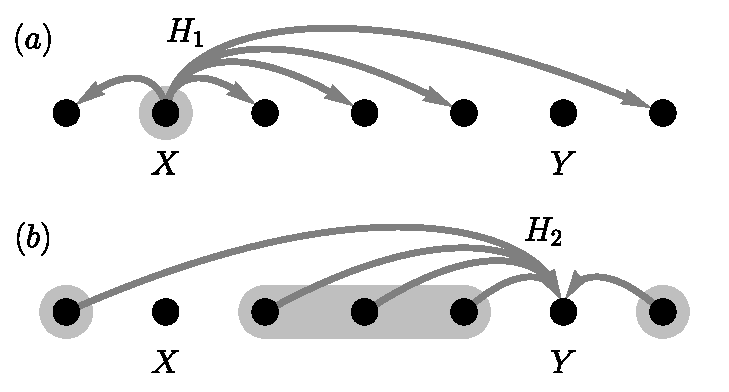
\includegraphics[width=0.9\linewidth]{figures/test_gong_protocol3.pdf}
\caption{A fast quantum state transfer protocol for a long-range Hamiltonian acting on a lattice of dimension $D=1$ with $N=7$ sites. The strengths of the hopping terms are bounded by a power-law $1/r^{\al}$ in the distance $r$. The active interactions in each time-step are depicted as directed edges with uniform weights. (a) The site $X$ is initially in the state $\ket{\psi}$ (gray circle), with the other (unoccupied) sites in state $\ket{0}$. Time-evolving by the Hamiltonian $H_1$ for time $\O{N^{\al/D-1/2}}$  (indicated by gray arrows) yields a superposition of the $\ket{0}^{\otimes N}$ state and a symmetric $\ket{W}$ state over the remaining $N-2$ sites. (b) Applying the Hamiltonian $H_2$ for the same duration of time completes the state transfer of $\ket{\psi}$ to the target site $Y$.}
\label{Fig_Gong}
\end{figure}

\sect{Saturating the free-particle bound}We now show that the bound in \cref{eq:tightbound} can be saturated by engineered Hamiltonians that can also be used to perform fast quantum state transfer. In particular, the protocol presented here has a state transfer time of $T = \O{N^{\alpha/D}/\sqrt{N}}$, which\dash for $\alpha\le D/2$\dash improves over the fastest-known state transfer protocol using long-range interactions \cite{Eldredge17}.

Our setup for the state transfer task is depicted in \cref{Fig_Gong}. We initialize a lattice with $N$ sites in a tensor product of unoccupied states $\ket{0}$ and some unknown normalized bosonic/fermionic state $\ket{\psi} = a\ket{0}+b\ket{1}$ on a single site $X$.
The goal of state transfer is to move $\ket{\psi}$ to the target site $Y$ after the system time-evolves by a $\ket{\psi}$-independent (but possibly time-dependent) Hamiltonian $H(t)$ \cite{NJ2014,Epstein17}.

The unitary time-evolution operator $U(T)$ can be said to implement state transfer in time $T$ if it satisfies the following condition:
\begin{align}
	\label{eq:fidelity}
	\left|\bra{0}_{X}\bra{0}^{\otimes N-2}\bra{\psi}_{Y} U(T)\ket{\psi}_{X}\ket{0}^{\otimes N-2}\ket{0}_{Y}\right| = 1.
 \end{align}
We refer to the left-hand side of \cref{eq:fidelity} as the \emph{fidelity} of the state transfer, which can be bounded directly by a Lieb-Robinson-type bound on $H(t)$ such as \cref{eq:tightboundeq} \cite{Epstein17}.

We label the sites that are not $X$ or $Y$ by $1,\dots,N-2$ and denote the furthest distance between any pair of sites by $L=\O{N^{1/D}}$. Our state transfer protocol is given by the following piece-wise time-independent Hamiltonian:
\begin{align}
\label{eq:protocol}
H(t)= \begin{cases}
	H_{1}=\frac{1}{L^{\al}} \sum_{i=1}^{N-2} c_{X}^{\dagger}c_{i}+\text{h.c.} & 0<t<\frac{T}{2},\\
	H_{2}=\frac{1}{L^{\al}} \sum_{i=1}^{N-2} c_{i}^{\dagger}c_{Y}+\text{h.c.} & \frac{T}{2}<t<T,
\end{cases}
\end{align}
where $T=\pi L^{\al}/\sqrt{N-2}$ is the total time for the protocol. Note that while $H(t)$ satisfies the constraint $|J_{ij}(t)|\le 1/r_{ij}^{\alpha}$ assumed in \cref{eq:corollary}, the corresponding $J_{ij}(t)$ terms do not actually vary with the distances between sites.

Evolving the initial state
$\ket{\Psi} \equiv \ket{\psi}_{X}\ket{0}^{\otimes N-2}\ket{0}_{Y}$  by $H_1$ for time $T/2$ yields the intermediate state
\begin{equation}
	e^{-i H_1 T/2}\ket{\Psi}= a \ket{0}^{\otimes N} + b\ket{0}_{X}\ket{W}\ket{0}_{Y}.
\end{equation}
Here, $\ket{W}= \frac{1}{\sqrt{N-2}}\sum_{i=1}^{N-2} c_{i}^{\dagger}\ket{0}^{\otimes N-2}$ is the W state over the $N-2$ remaining sites. Further evolving the state by $H_2$ for time $T/2$ yields the final state:
\begin{equation}
	e^{-i H_2 T/2}e^{-i H_1 T/2}\ket{\Psi}= \ket{0}_{X}\ket{0}^{\otimes N-2}(a \ket{0}_{Y}+ b\ket{1}_{Y}).
\end{equation}
Thus we have achieved perfect quantum state transfer in time $T = \O{N^{\al/D}/\sqrt{N}}$.
Note that the distance between $X$ and $Y$ on the lattice does not appear in the state transfer time.
    Setting $b=1$ in the above protocol leads to
\begin{equation}
    \expval{[c^\dagger_{X}(T),c_{Y}]}{\Psi} = \frac{1}{2}\int_{0}^{T}d\tau\sqrt{\sum_{i\in\Lambda}\left|J_{iX}(\tau)\right|^{2}}.
\end{equation}
Thus, the bound in \cref{eq:tightboundeq} is saturated up to a factor of 2.

It should be pointed out that, for $\al > D/2$, the above protocol requires a time that increases with $N$, which is slower than for the previous result in Ref.~\cite{Eldredge17}.
While that protocol has a state transfer time that is constant for $\alpha\le D$, it uses an engineered Hamiltonian with interactions, and therefore cannot be applied to systems of non-interacting particles.
In general, allowing interactions may increase the rate of information propagation, and proving a Lieb-Robinson-type bound in these situations requires a different approach.

\sect{Improved bound for general interacting systems}We now derive bounds on the signaling time that extend beyond free-particle Hamiltonians.
Without loss of generality, we study a generic interacting spin Hamiltonian $ 	H(t) = \sum_{i<j} h_{ij}(t)$ where $\|h_{ij}(t)\|\le 1/r_{ij}^{\alpha}$ and on-site interactions have been eliminated by going into an interaction picture.
We will bound the quantity $\|[A(t),B]\|$, where $A$ and $B$ are arbitrary operators supported on sets of sites $X$ and $Y$ respectively,  using the following Lieb-Robinson series \cite{HK}:
\begin{align}
	\label{eq:HKseries1}
	\|[A(t),B]\| &\le 2\|A\|\|B\||X||Y|\sum_{k=1}^{\infty}\frac{(2t)^{k}}{k!} \J^k(X,Y), \\
    \label{eq:hoppingterms}
	\J^k(X,Y) &\equiv \sum_{i_{1},\dots,i_{k-1}}J_{Xi_{1}}J_{i_{1}i_{2}}\dots J_{i_{k-1}Y}.
\end{align}
Here, $|X|$ stands for the number of sites $X$ acts on. Each term in \cref{eq:hoppingterms} represents a sequence of $k$ directed hops in the lattice that originates at site $X$ and ends at site $Y$.
For distinct sites $i$ and $j$, $J_{ij}=1/r_{ij}^{\al}$ represents a directed hop from $i$ to $j$.
For technical reasons, we set $J_{ii} = \sum_{j\ne i} J_{ij}$ \footnote{
The strength of the on-site hop $J_{ii}$ is defined this way for technical reasons that we explain in the Supplemental Material.}.

Since $J_{ij}$ decays slowly in $r_{ij}$ for $\alpha<D$, our improved bound on $\|[A(t),B]\|$ requires bounding each term in \cref{eq:hoppingterms} using a new summation technique \cite{SM} absent in previous efforts \cite{HK,Storch15}. This technique is particularly effective for tightening existing Lieb-Robinson bounds for strongly long-range interacting systems. The result (assuming $\alpha<D$) is:

\begin{equation}
\label{eq:newbound}
	\|[A(t),B]\| \le  2\|A\|\|B\||X||Y|\left(\frac{e^{\Theta(N^{1-\al/D})t}-1}{\Theta(N^{1-\al/D})r_{XY}^\al}\right).
\end{equation}
The factor $\Theta(N^{1-\alpha/D})$ \cite{bigO} comes from the total interaction energy per site given by $J_{ii}$.

We consider now the case of signaling between subsystems $X$ and $Y$ of a system $\Lam$ with $|X|,|Y|=\O{1}$.
We formally define $t_\text{si}$\dash the signaling time from $X$ to $Y$\dash as the smallest time $t$ such that for a fixed constant $\delta=\Theta(1)$, there exist unit-norm operators $A$ and $B$ supported on $X$ and $Y$ respectively such that $\|[A(t),B]\| > \delta$ \cite{Lashkari13}.
If we further assume that $X$ and $Y$ are separated by an extensive distance $r_{XY}=\Th{N^{1/D}}$, then the following lower bound holds for the signaling time:
\begin{equation}
	\label{eq:tsi}
	t_\text{si}=  \W{\frac{\log(N)}{N^{1-\al/D}}}.
\end{equation}
This bound supersedes the naive signaling-time bound of $t_\text{si}= \W{ 1/N^{1-\alpha/D}}$ one would obtain via normalization of interaction energy per site.
While we do not know of any examples that saturate this bound, it is the tightest-known signaling-time bound for strongly long-range interacting systems.
Indeed, the bound is close to being saturated in the limit of $\alpha\rightarrow D^-$, as the state transfer protocol in Ref.~\cite{Eldredge17} shows that $t_\text{si}=\O{\log(N)}$ can be achieved at $\alpha=D$. Unfortunately, generalizing our bound in \cref{eq:newbound} to the case of $\alpha=D$ leads to $t_\text{si}=\W{1}$ \cite{SM}, which is not saturated by Ref.~\cite{Eldredge17}.

\sect{Many-site signaling and scrambling bounds}Of recent interest in the fields of theoretical high-energy and condensed matter physics has been the phenomenon of quantum information scrambling \cite{Lashkari13,Swingle16,SS08,Hayden07,Xu18,Shenker14,Hosur16,Nahum18,Keyserlingk18,Roberts18,Gu17}.
Previous work on scrambling in power-law interacting systems has focused primarily on numerical analysis \cite{Pappalardi18,Zhou18}, whereas general mathematical results are lacking.
Only in all-to-all interacting systems (which can be treated as the limit $\al=0$) have Lieb-Robinson-type bounds been used to bound the scrambling time \cite{Lashkari13}.
Using the bound derived in \cref{eq:newbound}, we can prove a scrambling-time bound for systems with $0<\alpha<D$, a regime for which no better result is known.

To derive a bound on the scrambling time, we first derive a bound on the many-site signaling time. We define the ``many-site signaling time'' $t_\text{ms}$ to be the smallest $t$ required to signal from $X$ to a $Y$ that has extensive size.
Lieb-Robinson-type bounds such as \cref{eq:newbound} naturally limit the time for many-site signaling. However, a direct application of \cref{eq:newbound} to many-site signaling leads to a loose bound. Instead, a more refined technique that sums over all sites within the subsets $X$ and $Y$ yields a tighter bound \cite{Gong17}:
\begin{equation}
\label{refinedbound}
    \|[A(t),B]\|\le  2\|A\|\|B\|\sum_{i\in X, j\in Y}\frac{e^{\Theta(N^{1-\al/D})t}-1}{\Theta(N^{1-\al/D})r_{ij}^\al}.
\end{equation}
This bound reduces to \cref{eq:newbound} when $|X|,|Y|=1$.

The scrambling time $t_\text{sc}$  corresponds to the minimal time required for a system of $N$ spins on a lattice $\Lam$ to evolve from a product state to a state that is nearly maximally entangled on all subsystems of size $kN$ for some constant $0<k<\frac12$ \cite{Lashkari13}.
From this definition, it can be shown that any information initially contained in a finite-sized subsystem $S \subset \Lam$ is no longer recoverable from measurements on $S$ alone \cite{Lashkari13}.
That information is not lost, however, but can be recovered from the complement $\bar{S} = \Lam \setminus S$ of $S$ \cite{Hayden07,Cotler18}.
As a result, scrambling implies the ability to signal from $S$ to $\bar{S}$ \cite{Lashkari13}.
Thus, $t_\text{sc}$ is lower bounded by the time it takes to signal from a subset $S$ with size $\Theta(1)$ to its complement with size $\Theta(N)$, which corresponds to the many-site signaling time.

Using \cref{refinedbound}, we obtain the following scrambling-time bound for $0\le\alpha<D$:
\begin{equation}
    \label{eq:manysitebound}
    t_\text{sc}\ge t_\text{ms}= \W{ \frac{1}{N^{1-\al/D}}}.
\end{equation}
Note that this bound differs from \cref{eq:tsi} by a $\log(N)$ factor.
Additionally, although the bound on $t_\text{si}$ in \cref{eq:tsi} may allow further tightening, the bound on $t_\text{ms}$ in \cref{eq:manysitebound} cannot be generically improved for $0\le\alpha<D$.
To see this, we consider a long-range Ising Hamiltonian $H=\sum_{i\neq j}J_{ij}\sigma_{i}^{z}\sigma_{j}^{z}$, with $J_{ij}=1/r_{ij}^{\al}$.
For simplicity, we consider the subset $S$ to be a single site indexed by $i$ and construct operators $A=\sigma_{i}^{+}$ and $B=\bigotimes_{j\ne i}\sigma_{j}^{+}$ that are supported on $S$ and $\bar{S}$ respectively.
We can analytically calculate the expectation value of $[A(t),B]$ in an initial state $\ket{\psi}=\frac{1}{\sqrt{2}}[\ket{0}^{\otimes N}+\ket{1}^{\otimes N}]$ \cite{Gong17}:
\begin{equation}
    \label{eq:manysiteprotocol}
\bra{\psi}[A(t),B]\ket{\psi}=\sin(2t\sum_{j\ne i}J_{ij}).
\end{equation}
Using $J_{ij}=1/r_{ij}^{\al}$, we find that the signaling time of this protocol is $t=\O{N^{\al/D-1}}$ for $0\le\al<D$, which saturates the many-site signaling-time bound in \cref{eq:manysitebound} \footnote{A different protocol for many-site signaling was given in \cite{Eisert13}. That result yields a many-site signaling time of $t_\text{ms} =\O{N^{\al/D-1/2}}$, which does not saturate the bound in \cref{eq:manysitebound}.}.
This does not, however, imply that the corresponding scrambling-time bound is tight.
In fact, previous work suggests that fast scramblers in all-to-all interacting systems ($\alpha=0$) can scramble in time $t_\text{sc}=\O{\log(N)/\sqrt{N}}$ \cite{Lashkari13}
\footnote{We note that the example of a fast scrambler given in \cite{Lashkari13} does not strictly obey the normalization condition $\norm{h_{ij}(t)}\le 1/r_{ij}^{\alpha}$. This does not, however,
 weaken the claim that there is gap between our scrambling-time bound and the scrambling times of fast-scrambling systems}.
This suggests that future improvements to the scrambling-time bound may be possible.

\sect{Conclusions and Outlook}In this paper, we make several advances in bounding the signaling and scrambling times in strongly long-range interacting systems.
Our results suggest a number of possible future directions.
One is to find the optimal signaling-time bound for general strongly long-range interacting systems.
Previously, this has been an outstanding challenge; we now know of a free-particle bound that is tight for $\al \in [0,D/2]$ and a general bound that is nearly tight as $\alpha\rightarrow D^-$.
The search for the optimal bound for $\alpha\in [0,D]$ has thus been narrowed down significantly.
Another direction is to investigate how interactions can speed up signaling.
We expect weakly interacting systems to possess a similar signaling-time bound to our free-particle bound, as the dynamics in such systems can often be treated using spin-wave analysis \cite{Cevolani18}.
But for strongly interacting systems, it remains unclear how much speedup one can obtain over non-interacting systems.

Additionally, our bound for signaling to an extensive numbers of sites hints at a strategy for achieving a better scrambling bound.
In particular, the protocol that saturates our many-site signaling bound relies on an initial entangled state, whereas the definition of scrambling assumes that the system begins in a product state.
It may be possible to improve the scrambling-time bound by explicitly restricting our attention, when bounding $t_\text{ms}$, to initial product states.

Finally, we expect that the improved Lieb-Robinson-type bounds derived in this work may lead to a better understanding of the spreading of out-of-time-order correlators \cite{Luitz19}, the growth of entanglement entropy \cite{Gong17}, and thermalization timescales \cite{Nandkishore15} in strongly long-range interacting systems.

In addition, there are connections between Lieb-Robinson-type bounds and the critical scaling of the defects appearing in a quantum system driven across its quantum critical point (the celebrated Kibble-Zurek (KZ) mechanism).
It remains an open question whether the KZ hypothesis can be shown to hold for strongly long-range systems.


% \chapter{Implementing a fast unbounded quantum fanout gate using power-law interactions}
\label{ch:qfo}
In the circuit model for quantum computation, the depth of a quantum circuit is given by the number of layers of non-overlapping quantum gates it contains.
In typical quantum systems, coherence times are a limitation, so low-depth circuits prioritized for the regime of noisy intermediate-scale quantum computers are more desirable \cite{Preskill2018}.
Various proposed models of quantum computation are equivalent up to polynomial overhead, making the definition of the complexity class $\BQP$ insensitive to the model of computation \cite{Bernstein1993,Raussendorf2001,Raussendorf2003,Hoyer2005}.

However, these models can differ in the precise complexity of operations.
As a drastic example, suppose we are given access to a fast unbounded fanout gate
represented by the map
$\ket{x} \ket{y_1} \ket{y_2} \dots$\,$\mapsto$\,$\ket{x}\ket{y_1 \oplus x} \ket{y_2 \oplus x} \cdots$
where the $\oplus$ operator denotes bitwise XOR (bit $y_i$ is flipped if $x$\,$=$\,$1$ and not flipped otherwise). This operation is a reversible analog of a gate that copies $x$ to registers $y_1, y_2, \dots$.
By ``unbounded,'' we mean that there is no limit on the number of bits that can be targeted by this operation.

The unbounded fanout gate makes it possible for constant-depth circuits to perform a number of fundamental quantum arithmetic operations \cite{Hoyer2005}.
Furthermore, unbounded fanout can also reduce the quantum Fourier transform (QFT)---a subroutine of a large class of quantum algorithms, including most famously Shor’s algorithm for integer factorization \cite{Shor1997}---to constant depth as well.
In fact, it enables implementing the entirety of Shor's algorithm by constant-depth circuits with access to a polynomial amount of classical pre- and post-processing \footnote{While the rate-limiting step for factoring is actually modular exponentiation, it is possible to implement this subroutine in logarithmic quantum depth with a polynomial number of classical gates as a pre-computation step, using a standard universal gate set for quantum computing \cite{Cleve2000}. Using the unbounded fanout gate, the quantum circuit for modular exponentiation can be reduced to constant depth as well \cite{Hoyer2005}.}.

While the unbounded fanout gate is clearly a powerful resource for quantum computation, its efficient implementation in physically realizable architectures has not been studied in great depth.
In the standard circuit model---where one may apply single-qubit and two-qubit gates from a standard gate set on arbitrary non-overlapping subsets of the qubits---a fanout gate on $n$ qubits can be implemented optimally in $\Th{\log{n}}$-depth \cite{bigO,Broadbent2009a}.
One may also consider the Hamiltonian model, in which one may apply single-qubit and two-qubit Hamiltonian terms.
In particular, in the Hamiltonian model with all-to-all unit-strength interactions, one can implement the fanout gate in constant time \cite{Fenner2003,Fenner2004}.
However, the assumption of being able to directly apply interactions between two arbitrarily distant qubits does not hold in practice for large quantum computing architectures \cite{Monroe2014,Linke2017,Bapat2018,Childs2019c}.
Mapping these circuits to restricted architectures inevitably leads to overheads and potentially even different asymptotic scaling.
In $d$-dimensional nearest-neighbor architectures, for example, the unbounded fanout gate can only be implemented unitarily in depth $\Th{n^{1/d}}$ \cite{Rosenbaum2013}.
And while there exist protocols that can implement the fanout gate in constant depth on these architectures \cite{Pham2013}, these proposals require intermediate measurements along with classical control---a resource that may be inaccessible in certain near-term experimental systems \cite{Arute2019}.
The overheads resulting from such physical restrictions could therefore limit the potential asymptotic speed-up from a fast quantum fanout.

Systems with power-law interactions, however, present an opportunity for realizing these speed-ups.
Specifically, for a lattice of qubits in $d$ dimensions, the interaction strengths between pairs of qubits separated by a distance $r$ are weighted by a power-law decaying function $1/r^\alpha$.
These long-range interactions are native to many experimental quantum systems and have attracted interest as potential resources for faster quantum information processing. Examples of long-range interactions include dipole-dipole and van der Waals interactions between Rydberg atoms~\cite{Saffman2010,Weimer2012}, and dipole-dipole interactions between polar molecules~\cite{Yan2013} and between defect centers in diamond~\cite{Yao2012,Weimer2012}.
Previous works have explored the acceleration of quantum information processing using strong and tunable power-law interactions between Rydberg states~\cite{Isenhower2011,Molmer2011,Petrosyan2017,Gulliksen2015,Muller2009,Young2020,Levine2019}, which can implement $k$-local gates that control or target simultaneously $k \gg 10$ qubits.
Those gates still have a finite spatial range and can therefore only give a constant-factor speed-up over nearest-neighbor architectures.
Recently, Refs.~\cite{Eldredge2017,Guo2020,Tran2020hierarchylinearlightcones,kuwaharaStrictlyLinearLight2020} gave protocols that take advantage of power-law interactions to quickly transfer a quantum state across a lattice.
As we will show, it is also possible to leverage the power of these interactions to implement quantum gates asymptotically faster than is possible with finite-range interactions \footnote{We note that in Refs.~\cite{Maslov2018,Lu2019}, it was shown that the unbounded quantum fanout could be implemented in trapped-ion systems using a global Molmer-Sorensen gate.
    However, those methods lead to gate durations that scale superlinearly in the system size in order to achieve a certain value of state fidelity and, as such, do not yield an asymptotic speed-up.}.

In this Letter, we propose a protocol for implementing the unbounded fanout gate quickly using engineered Hamiltonians with power-law interactions.
As an application of this protocol, we show that simulating long-range systems with $\al$\,$\le$\,$2d$ for polylogarithmic time or longer is classically intractable, if factoring is classically hard.
As a complement to our upper bounds on the fanout time, we also develop a technique that allows us to prove the tightest-known lower bounds for the time required to implement the QFT and unbounded fanout in a general lattice architecture.

\section{Protocol for fast fanout using long-range interactions}
To perform a fanout gate on $n$ logical qubits, we
employ as subroutines modified versions of the state transfer protocols from Refs.~\cite{Eldredge2017} and \cite{Tran2021a} to generate a many-body entangled state in $\O{\polylog(n)}$ time using long-range interactions with $\al$\,$<$\,$2d$.

As an intermediate step, both state-transfer protocols ``broadcast'' a single-qubit state into the corresponding Greenberger–Horne–Zeilinger (GHZ)-like state:
\begin{equation}
    \label{eq:longrangebroadcast}
	(\psi_0 \ket{0} + \psi_1 \ket{1})\otimes \ket{0 0 \dots 0} \mapsto \psi_0 \ket{0 0  \dots 0} + \psi_1 \ket{1 1 \dots 1},
\end{equation}
where $\psi_0, \psi_1$\,$\in$\,$\mathbb{C}$ and $|\psi_0|^2$\,$+$\,$|\psi_1|^2$\,$=$\,$1$.
In the case of Ref.~\cite{Eldredge2017}, this long-range broadcast is achieved by performing a sequence of cascaded controlled-\textsc{Not} (\textsc{CNot}) gates---similar to the standard gate-based implementation of the unbounded fanout gate.
The \textsc{CNot} gate from qubit $i$ to qubit $j$ can be implemented by a Hamiltonian $H_{ij}$\,$=$\,$h_{ij} \ketbra{1}_i$\,$\otimes$\,$X_j$ acting for time $t$\,$=$\,$\pi/(2h_{ij})$, up to a local unitary.
Applying a Hamiltonian $H(t)$\,$=$\,$\sum_{ij} H_{ij}(t)$, which variously turns on/off interactions between pairs of qubits at different times, allows one to implement the broadcast in \cref{eq:longrangebroadcast}.

By using Hamiltonians with long-range interactions $h_{ij}$ satisfying $\norm{h_{ij}}$\,$\le$\,$1/r_{ij}^\al$, it is possible to implement the broadcast operation asymptotically faster than with short-range interactions---a statement that we will prove rigorously later in the text.
For a system of $n$ qubits, Refs.~\cite{Eldredge2017} and \cite{Tran2021a} showed that this broadcast time depends on the power-law exponent $\al$ and the dimension of the system $d$ as follows:
\begin{equation}
\label{eq:statetransfertimes_new}
	\tghz =
  \begin{cases}
    \O{n^0} & \alpha < d
    \\ \O{\log n} & \alpha = d
    \\ \O{\log^{\kappa_\alpha} n }& \alpha \in (d,2d)
    \\ \O{e^{\gamma\sqrt{\log n}}}& \al = 2d
    \\ \O{n^{\min(\al/d - 2,1)}} & \alpha > 2d,
  \end{cases}
\end{equation}
for constants $\gamma = 3\sqrt{d}$ and $\kappa_\alpha = \log 4/\log(2d/\alpha)$.
We term the broadcast time $t_{\text{GHZ}}$, since it corresponds to the GHZ-state-construction time when $\psi_0$\,$=$\,$\psi_1$\,$=1/\sqrt{2}$.
This long-range broadcast is not the same as fanout because it requires that all intermediary qubits (besides the first qubit) be initialized in the $\ket{0}$ state.
However, as we now show, it is possible to adapt the broadcast protocol to implement the fanout gate in time $\tghz$ using $n$ ancillary qubits.

\begin{figure}[t]
\centering
    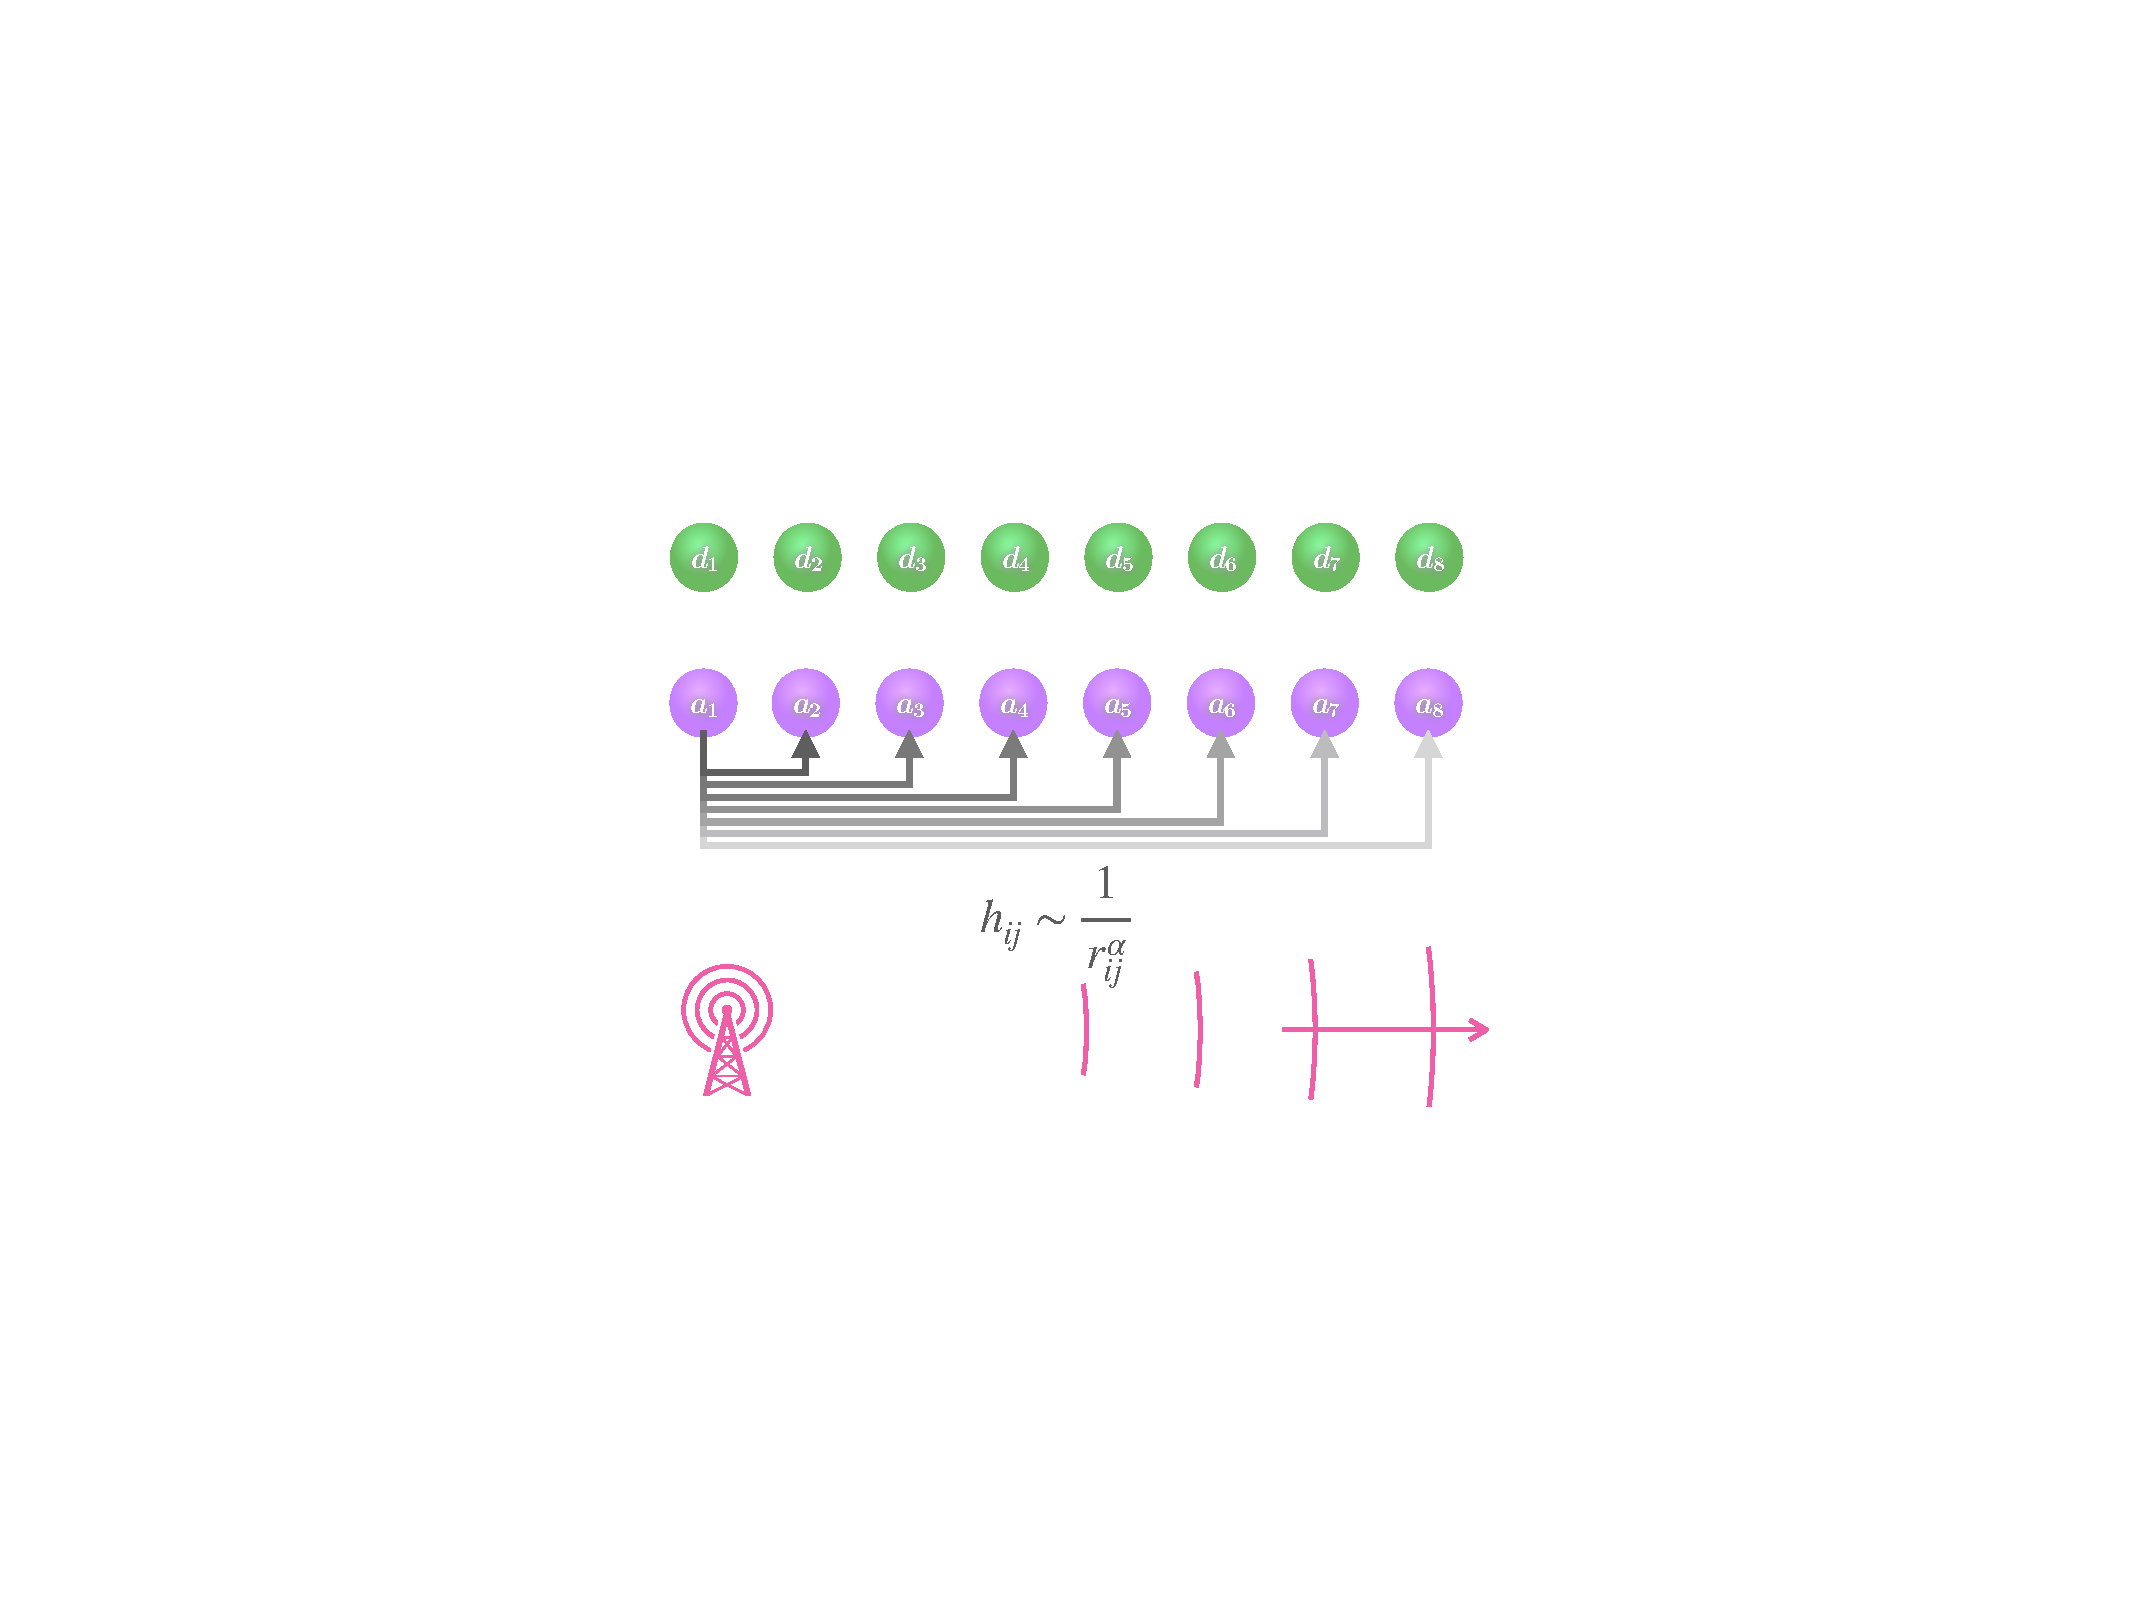
\includegraphics[scale=0.45]{figures/fanoutgate.pdf}
\centering
  \caption{A protocol for a fast unbounded quantum fanout gate using long-range interactions, depicted here for a 1D lattice.
  The layout consists of a chain of data qubits, along with their adjacent ancillary qubits that are initialized to $\ket{0}$.
  (a) The first step is a local controlled-\textsc{Not} (\textsc{CNot}) gate from $\ket{d_1}$ to $\ket{a_1}$.
  (b) The application of the long-range ``broadcast'' from $\ket{a_1}$ to the rest of the ancillary qubits $\ket{a_i}$ creates a GHZ-like state in Eq.\,(\ref{eq:longrangebroadcast}) for the ancillary qubits together with the first data qubit.
  (c) We apply \textsc{CNot} gates from ancillary qubit $\ket{a_i}$ to the data qubit $\ket{d_i}$, which can be done in parallel. After this step, we reverse process (b) and process (a) to return the ancillary qubits to $\ket{0}$ (not redrawn here). }
  \label{fig:broadcast}
\end{figure}

Consider a system of $n$ data qubits arranged on a $d$-dimensional lattice.
Furthermore, assume there are $n$ ancillary qubits, each located adjacent to one of the original qubits.
We denote the qubits as $\ket{d_1}, \ket{d_2}, \dots, \ket{d_n}$ and $\ket{a_1}, \ket{a_2}, \dots, \ket{a_n}$ for data and ancilla, respectively.
Suppose we want to perform fanout with $\ket{d_1}$ as control, and that all ancillae are guaranteed to be in state $\ket{0}$.
Then the sequence of operations in \cref{alg:fastfanout} (also depicted graphically in \cref{fig:broadcast}) implements the fanout operation.

In addition to accomplishing fanout, this protocol returns the ancillary qubits to the $\ket{0}$ state.
Modulo the $\O{n}$ short-range operations that can be done in parallel in a single time step, the protocol requires time $2 t_\mathrm{GHZ}$.
Hence, it can implement the fanout gate in time that is constant for $\alpha$\,$<$\,$d$, polylogarithmic for $d$\,$\le$\,$\alpha$\,$<$\,$2d$, and polynomial for $\alpha$\,$>$\,$2d$.

\begin{algorithm}[H]
% \renewcommand{\thealgorithm}{}
  \caption{Implementing fanout with long-range interactions}
  \label{alg:fastfanout}
  \begin{algorithmic}[1]
   \State Initialize ancillary qubits: $\ket{a_i}$\,$\gets$\,$\ket{0}$ for $i$\,$=$\,$1$ to $n$
  \State \textsc{CNot}($\ket{d_1}$\,$\ra$\,$\ket{a_1}$)
  \Statex $\bigtriangledown$ Apply broadcast operation as shown in \cref{eq:longrangebroadcast} to ancillae:
  \State \textsc{LongRangeBroadcast}($\ket{a_1}$\,$\ra$\,$\ket{a_2},\dots,\ket{a_n}$)
  \Statex $\bigtriangledown$ \textbf{parfor} indicates that \textbf{for}-loop can be implemented in \textbf{par}allel
  \ParFor {$i$\,$=$\,$2$ to $n$}
    \State \textsc{CNot}($\ket{a_i}$\,$\ra$\,$\ket{d_{i}}$)
    \Comment{\parbox[t]{.45\linewidth}{{Transfer} fanout to data qubits}}
  \EndParFor
  \Statex $\bigtriangledown$ Apply broadcast operation in reverse to uncompute ancillae
  \State \textsc{ReverseLongRangeBroadcast}($\ket{a_2},\dots,\ket{a_n}$\,$\ra$\,$\ket{a_1}$)
  \State \textsc{CNot}($\ket{d_1}$\,$\ra$\,$\ket{a_1}$)
  \end{algorithmic}
\end{algorithm}

We briefly comment on the constant-depth implementation of the QFT and Shor's algorithm using the unbounded fanout gate.
An $n$-qubit QFT circuit can be performed with $\O{n\log n}$ gates to $1/\text{poly}(n)$ precision \cite{Coppersmith94}.
Using unbounded fanout, the circuit can be reduced to constant depth with $\O{n\log n}$ ancillary qubits \cite{Hoyer2005}.
We note that including these ancillae in the lattice would not change the asymptotic scaling of our protocol for $\al$\,$<$\,$2d$, since $\tghz$ is $\O{\polylog(n)}$ in this regime.

We also remark on the potential ways of performing the fast fanout gate experimentally.
One method would be to use two different qubit realizations for the data and ancillary qubits,  with the former interfacing with the latter through local interactions.
For example, one may consider a system of fermionic alkaline-earth atoms, with each atom's electron on the clock transition acting as an ancillary qubit, its nuclear spin as the data qubit, and with long-range Rydberg-Rydberg interactions between electrons.
In this heterogeneous case, the $n$ $\textsc{CNot}$ gates between the data and ancilla qubits of our protocol would be straightforward to implement in parallel \cite{Gorshkov2009}.
Alternatively, one may consider implementing the protocol entirely in a system of Rydberg atoms using power-law interactions of different strengths.
This could be done using a gate based on %diagonal
van der Waals interactions ($\al = 6$) to implement the short-range $\textsc{CNot}$ gates between data and ancilla qubits, and then rotating into a new basis in order to implement the long-range broadcast interaction using dipole-dipole interactions ($\al = 3$).
We provide more discussion on the implementation of the protocol in the Supplemental Material \cite{SM}.

\section{Intractability of classical simulation of long-range systems with $\al$\,$<$\,$2d$}
As a corollary, the protocol shows that long-range interacting systems with $\al$\,$<$\,$2d$ evolving for time polylogarithmic in $n$ or longer are difficult to simulate classically in the worst case.
% By this we mean that in order to approximately sample from the time-evolved state to within constant total-variation-distance error $\varepsilon$, a classical computer would require time at least superpolynomial in the system size \cite{note_constanterror}.
The argument operates by a complexity-theoretic reduction from integer factoring, a problem that is assumed to be difficult for classical computers with the ability to use random bits (\textsc{Factoring} $\notin$\,$\BPP$).
This assumption suggests that the simulation of long-range systems could provide an avenue towards a potentially useful experimental demonstration of quantum computational advantage.

The argument proceeds as follows.
The time required to implement the fanout gate using \cref{alg:fastfanout} is $\O{\polylog(n)}$ for $\al$\,$<$\,$2d$.
It is possible to implement Shor's order-finding algorithm in time $\O{t_\mathrm{FO}}$ using a small amount of classical pre-processing (polynomial in $n$) \cite{Cleve2000,Hoyer2005}.
Using the ability to sample from the output of the order-finding algorithm to error $\varepsilon$\,$<$\,$0.4$\,$<$\,$4/\pi^2$, classically efficient post-processing can output a factor of an $n$-bit integer with probability $\W{1}$ \cite{Shor1997}.
Therefore, if it were possible to efficiently sample from the output distribution in long-range systems with $\al$\,$<$\,$2d$ for evolution-time $t$\,$=$\,$\mathcal{O}(\log n)$, then it would be possible to factor $n$-bit integers efficiently as well.
The best classical algorithm currently known for factoring an $n$-bit integer takes runtime $\exp[\mathcal{O}(\sqrt{n \log n})]$ \cite{Lenstra1992} and the problem is widely believed to be classically intractable.
This stands in contrast to systems with finite-range interactions in 1D, for which efficient classical simulation is possible up to any time satisfying $t$\,$\leq$\,$\O{\log n}$ \cite{Osborne2006}.
Under the complexity assumption mentioned above (\textsc{Factoring} $\notin$\,$\BPP$), we have shown that this result is not fully generalizable to long-range interacting systems with $\al$\,$<$\,$2d$\footnote{We note that a similar result could have been achieved using the fact that constant-depth quantum circuits with two fanouts are not classically simulable unless $P = PP$ \cite{Takahashi2014}.}.


%%%%%%Lower bounds on the time required to implement QFT and fanout%%%%%%%

\section{Lower bounds on the time required to implement QFT and fanout}
In previous sections, we found upper bounds to the time required to implement fanout---and by corollary, the QFT.
As a way to benchmark our long-range protocol, we now proceed to discuss lower bounds for implementing fanout and the QFT.
Recall that the protocol in \cref{alg:fastfanout} can implement fanout in time $\tghz$, which scales as $\O{\polylog(n)}$ for long-range systems with $\alpha$\,$<$\,$2d$.
In this section, we show that such fast asymptotic runtimes cannot be achieved in architectures with strict locality constraints.

In Ref.\,\cite{Maslov2007}, Maslov showed that a specific way of implementing the QFT requires $\W n$ depth on the 1D  nearest-neighbor architecture, though this does not rule out other QFT implementations with potentially sublinear depth.
Here, we devise a technique that yields a lower bound of $\W {n^{1/d}}$ for the time required to perform a QFT in the Hamiltonian model.
This result strengthens and generalizes Maslov's bound to higher dimensions and to the Hamiltonian model.
In addition, we show that the same lower bound applies even to circuits that perform the QFT approximately.

Our $\W {n^{1/d}}$ lower bound holds for any lattice system with finite velocities of information spreading, which include short-range interactions (i.e., finite-ranged or exponentially decaying) and power-law interactions with $\al$\,$>$\,$2$ in one dimension or $\alpha$\,$>$\,$2d$\,$+$\,$1$ for $d$\,$>$\,$1$ \cite{Lieb1972,Chen2019,kuwaharaStrictlyLinearLight2020}.
Combined with our results above, this implies that systems with long-range interactions with $\al$\,$<$\,$2d$ can implement the QFT and fanout asymptotically faster than more weakly interacting systems.

The intuitive idea behind our proof is that the QFT unitary can spread out operators in a certain precise sense, a task that can be bounded by the ``Frobenius-norm light cone'' of Ref.\,\cite{Tran2020hierarchylinearlightcones}.
The fact that this light cone imposes a finite speed limit on information propagation in short-range interacting systems implies that the minimum time $t_2(r)$ required for operator-spreading is proportional to the distance between qubits $r$.
This constrains the implementation time for the QFT, denoted $t_\mathrm{QFT}$, by $\W {n^{1/d}}$, from which the circuit-depth lower bound follows.
The same Frobenius-norm bound also constrains the time required to implement the approximate QFT (AQFT).

We consider the $4^n$-dimensional vector space of $n$-qubit operators for which the set of Pauli operators $\{I,X,Y,Z\}^{\otimes n}$ forms a basis.
We quantify operator spreading outside a region of radius $r$ as follows.
Taking an operator $|O)$ initially supported on site 1, we measure the weight of its time-evolved version, $|O(t))$, on sites at distance $r$ (and beyond) using a \emph{projection} operator $\mathcal{Q}_{r}$, which projects onto strings of Pauli operators that act nontrivially on at least one site at distance $r$ or greater.
We measure the weight of this projected operator $|O_r)$\,$\coloneqq$\,$\mathcal{Q}_{r}|O(t))$ via the (squared) normalized Frobenius norm $\norm{O_r}_F^2$\,$\coloneqq$\,$\Tr(O_r^\dag O_r)/2^n$, which coincides with the Euclidean norm over the operator space, $(O_r|O_r)$ \footnote{See Ref.\,\cite{Tran2020a} for a more precise definition.
    We note that our projector $\mathcal{Q}_r$ is a variation on the $\mathbb{Q}_r$ used in {Ref.\,\cite{Tran2020a}}.
    Specifically, for $d=1$, they are related via $\mathcal{Q}_r = \sum_{x:\,|x|\ge r} \mathbb{Q}_x$.}.
We define $t_2(r)$ to be the minimal time after which $\norm{O_r}_F^2$ is able to achieve a predetermined constant value \cite{Tran2020hierarchylinearlightcones}.
% on sites at distance $r$ or beyond. \cite{note_t2r}.

We show that operators spread by the action of the QFT can have high weight on distant regions,
which implies that $t_\mathrm{QFT}$\,$\geq$\,$t_2(r)$.
Recall that the QFT operator on $n$ qubits is defined as $U_\mathrm{QFT} \coloneqq \sum_{y,z=0}^{2^n-1} \ketbra{y}{z} {\omega^{yz}}/{\sqrt{2^n}}$, where $\ket{y}$ $(\ket{z})$ is an $n$-qubit state that encodes the binary representation of $y$ ($z$) and $\omega = e^{2\pi i/2^n}$.
Then the following lemma holds:
\begin{lemma*} \label{lem_qft_weight}
Let $U_\mathrm{QFT}$ be the QFT operator on $n$ qubits arranged in a $d$-dimensional lattice such that the first and $n$-th qubits are located a distance $r$\,$=$\,$\Theta(n^{1/d})$ apart.
Then $U_\mathrm{QFT}^\dag Z_1 U_\mathrm{QFT}$\,$=:$\,$Z_1' $ is an operator with at least constant weight at distance $r$.
\end{lemma*}

We defer the (short) proof of this Lemma to the Supplementary Material \cite{SM}.
As a result of the Lemma, $t_\mathrm{QFT}$ follows the light cone defined by the normalized Frobenius norm, which is at least as stringent as the Lieb-Robinson light cone.
This leads directly to the following theorem:
%
% \begin{proof}
% We explicitly compute the weight of the operator $Z_1'$ on site $n$.
% define $\omega$\,$:=$\,$e^{2\pi i/2^n}$.
% The QFT operation on $n$ qubits is defined as $\sum_{y,z=0}^{2^n-1} \ketbra{y}{z} {\omega^{yz}}/{\sqrt{2^n}}$, where we interpret the bit string $y_1, y_2, \ldots, y_n$ as a binary representation of a number $y$\,$\in$\,$\{0,1,\ldots, 2^n -1\}$ in the canonical ordering, i.e.\ $y$\,$=$\,$y_1 2^{n-1}$\,$+$\,$y_2 2^{n-2}$\,$+$\,$\cdots$\,$+$\,$y_n$.
% The inverse of the QFT is obtained simply by taking $\omega$\,$\rightarrow$\,$\omega^{-1}$.
% First, we compute
% \begin{align}
% Z_1' &= \sum_{x,y,z=0}^{2^n-1} \ketbra{z}{y} \frac{\omega^{-z y}(-1)^{y_1} \omega^{yx}}{2^n} \ketbra{y}{x}.
% \end{align}
% We divide the sum over $y$ into two cases, $y_1$\,$=$\,$0$ and $y_1$\,$=$\,$1$:
% \begin{align}
% Z_1' &= \frac{1}{2^n}\sum_{x,z=0}^{2^n-1} \ketbra{z}{x} \left(\sum_{y:\, y_1 = 0} \omega^{(x-z) y} - \sum_{y:\, y_1= 1} \omega^{(x-z) y}\right).
% \end{align}
% We can compute these sums separately, giving
% \begin{align}
% \label{eq:zoneprime}
% Z_1' = \frac{1}{2^{n-1}}\sum_{x\neq z}\ketbra{z}{x} \frac{1 - (-1)^{(x-z)}}{1-\omega^{x-z}}.
% \end{align}
% The nonzero terms in the sum on the right-hand side of \cref{eq:zoneprime} occur when $x-z$ is odd, i.e., when $x_n$\,$-$\,$z_n$\,$=$\,$1 \bmod 2$.
% Therefore, the only terms that remain are off-diagonal on qubit $n$ or, equivalently, contain only the $X_n$ or $Y_n$ Pauli operators.
% This implies that $Z_1'$ has all its weight on operators acting nontrivially at distance $r$---formally, that $\mathcal{Q}_r |Z_1')$\,$=$\,$|Z_1')$.
% \end{proof}

%
\begin{theorem*}  \label{thm:QFTlowerbounds}
  For systems with finite-range or exponentially-decaying interactions in $d$ dimensions, the time required to implement the QFT unitary is lower bounded by $t_\mathrm{QFT}$\,$= $\,$\W{r}$, where $r$\,$=$\,$\Theta(n^{1/d})$ is the distance between the first and $n$-th qubits.

  For systems with long-range interactions, the Lieb-Robinson light cone gives the following bounds \cite{kuwaharaStrictlyLinearLight2020,Tran2019a,Hastings2006,Tran2021b}:
  \begin{align}
  \label{eq:LRlowerbounds}
   t_\mathrm{QFT} =
   \begin{cases}
      \W{1}, & \al = d
      \\ \W{\log r}, & \alpha \in (d,2d]
      \\ \W{r^{\alpha-2d}}, & \alpha \in (2d,2d+1]
      \\ \W{r}, & \alpha > 2d + 1.
    \end{cases}
  \end{align}
  The Frobenius light cone gives the following (tighter) bounds \cite{Kuwahara2021,Chen2021Frobenius}:
  \begin{align}
  \label{eq:Froblowerbounds}
   t_\mathrm{QFT} =
   \begin{cases}
      \W{r^{\frac{2\al-2d}{2\alpha-d+1}}}, & \al \in (d,2d]
      \\ \W{r^{\alpha -1}}, & \alpha \in (1,2], d=1
      \\ \W{r}, & \alpha > 2, d=1.
   \end{cases}
  \end{align}
\end{theorem*}
%
We note that the lower bounds in the Theorem also apply to the fanout time, $t_\mathrm{FO}$, through the observation that fanout also performs operator spreading (using $X_1$ instead of $Z_1$).
We emphasize that these bounds pertain to the Hamiltonian model, where commuting terms can be implemented simultaneously and state transfer could in theory be done in $o(1)$ time for sufficiently small $\alpha$.

We observe that the QFT can implement quantum state transfer as well.
The goal of state transfer is to find a unitary $V$ such that
$V \bigl(\ket{\psi} \otimes \ket{0}^{\otimes n-1}\bigr)$\,$=$\,$\ket{0}^{\otimes n-1}$\,$\otimes $\,$\ket{\psi}$ \cite{Eldredge2017,Epstein2017}.
The unitary $V$\,$=$\,$H^{\otimes n} U_\mathrm{QFT}$ (where $H$ represents the single-qubit Hadamard gate) satisfies this definition of state transfer.

For the AQFT, the lower bound follows in a similar fashion.
The circuit that implements the QFT approximately with error $\varepsilon$ can be represented by a unitary $\tilde{U}_\mathrm{QFT}$ such that $\|U_\mathrm{QFT}-\tilde {U}_\mathrm{QFT}\|\leq \varepsilon$ \cite{Cleve2000}.
In the Supplemental Material, we show that the operator $\tilde {U}_\mathrm{QFT}^\dag Z_1 \tilde {U}_\mathrm{QFT}$ also has large support on sites beyond distance $r$ as well, implying that the lower bounds in \cref{eq:LRlowerbounds,eq:Froblowerbounds} also hold for the AQFT.

\section{Conclusions and Outlook}
In
summary, we have developed a fast protocol for the unbounded fanout gate using power-law interactions.
For $\al$\,$\le$\,$2d$, the protocol can perform the gate parametrically faster than is possible with short-range interactions.
In particular, for experimentally realizable dipole-dipole interactions with $\al$\,$=$\,$3$ in two and three dimensions, as well as van der Waals interactions with $\al$\,$=$\,$6$ in three dimensions, the fast fanout protocol allows the quantum Fourier transform and Shor's algorithm to be performed in time that scales subpolynomially in the number of qubits.
As a corollary, we showed that the classical simulation of long-range systems with $\al$\,$<$\,$2d$ for time $t$\,$=$\,$\O{\polylog(n)}$ is at least as difficult as integer factorization, which is believed to be intractable in polynomial time classically.

To benchmark our protocol, we developed a new and general approach for lower-bounding the time required to perform a given quantum algorithm that is independent of its implementation as a quantum circuit.
In particular, we derive a $\W{n^{1/d}}$ lower bound on the time required to implement quantum fanout—--as well as the exact and approximate QFTs---for all systems constrained by a linear light cone.
In doing so, we used the state-of-the-art Frobenius bounds from \cite{Tran2020hierarchylinearlightcones,Kuwahara2021,Chen2021Frobenius}, which have been shown to be tighter than the Lieb-Robinson bound in the regimes of $\al$ in which they hold.
While the Lieb-Robinson bound has been shown to be saturable for all $\al$\,$\ge$\,$d$ (up to logarithmic factors), the corresponding result for the Frobenius bound remains unknown.
For higher dimensions, the conjectured Frobenius light cone is $t$\,$=$\,$\W{r^{\alpha-d}}$ for $d$\,$<$\,$\al$\,$<$\,$d+1$ \cite{Chen2021Frobenius}.
If this generalization of the Frobenius bound were to hold, our lower bounds on the circuit complexity of QFT and fanout would immediately generalize.

As a final remark, we have derived our lower bounds on $t_\textrm{QFT}$ under the assumption that the first and last qubits of the QFT are separated by a distance of $r$\,$=$\,$\Theta(n^{1/d})$.
However, other mappings of computational qubits to lattice qubits could potentially lead to faster implementations.
For example, consider the mapping onto a one-dimensional chain of qubits wherein the second half of the chain is interleaved in reverse order with the first half \footnote{Specifically, for even $n$, this mapping is defined by $q_i\mapsto q_{2i-1}$ for $i \le n/2$ and $q_i\mapsto q_{2(n-i+1)}$ for $i > n/2$.}.
Applying the QFT to a product state in this layout results in a state with two-qubit correlations that decay exponentially in the distance between the qubits.
In this case, our lower bound techniques cannot rule out the possibility of $t_\textrm{QFT}$\,$=$\,$o(n)$ for short-range interacting Hamiltonians.
This suggests that $t_\textrm{QFT}$ could depend strongly on qubit placement.
Given that the QFT is typically used as a subroutine for more complex algorithms, it may not always be possible to reassign qubits without incurring costs elsewhere in the circuit.
Still, it would be interesting to investigate whether careful qubit placement could yield a faster QFT.


\section{Clustering of steady-state correlations in open systems with long-range interactions}

While the speed of information transfer is always bounded by the speed of light, many quantum platforms operate in a non-relativistic regime where typical velocities are far below this threshold.
Nevertheless, the  Schr\"odinger equation admits fundamental limits to the rate  at which correlations  can spread throughout the system.
Such bounds are known as Lieb-Robinson bounds and are connected to a diverse array of phenomena, including the decay of correlations in the ground state \cite{Hastings2006}, generation of topological order \cite{Bravyi2006, Bravyi2010}, efficiency of classical/quantum simulation \cite{Osborne2006,Tran2019a}, hardness of bosonic sampling tasks \cite{Deshpande2018}, heating rates in periodically driven Floquet systems \cite{Abanin2015,Tran2019b}, and signatures of quantum chaos \cite{Lashkari2013,Guo2019}.

To date, most  formulations of Lieb-Robinson bounds apply to closed systems that evolve  via a unitary time-evolution operator.
In such systems, recent advances have proved tight information-transfer bounds for interaction ranges that span the whole spectrum from local \cite{ChenLucas2021graphtheory,WangHazzard2020} to highly non-local regimes \cite{Tran2019a,Chen2019,kuwaharaStrictlyLinearLight2020,Tran2021b}, and have been saturated via explicit state-transfer protocols \cite{Eldredge2017,Tran2020hierarchylinearlightcones,Tran2021}.
While a complete picture for quantum information transfer has emerged for closed quantum systems,  the analogous question for systems that evolve \textit{non-unitarily} in time remains less well understood.
For a broad range of quantum platforms (including noisy quantum simulators), interactions with a  larger environment are unavoidable and must be taken into account to accurately describe dynamics.
While progress in this direction has been made \cite{poulin2010, descamps2013, cubitt2015, Kastoryano2013, Sweke2019}, the question of how the fundamental rate of information transfer differs for systems that interact with some larger environment remains unanswered.

Indeed, the notion of a  Lieb-Robinson bound in an open system may seem \textit{a priori}  surprising from the point of view of quantum trajectories \cite{Knight1998}. In this picture,  in a time-step $dt$ the system's wavefunction either evolves via a non-unitary evolution operator, or a quantum jump discontinuously  alters the state.
A specific  trajectory belonging to a spatially-local Hamiltonian with local dissipation can transfer information faster than  the limit set by the Hamiltonian's Lieb-Robinson bound \cite{Ashida2018}. Intuitively, this is because conditioning on measurements is an inherently nonlocal process.  As an extreme example, it is possible to create a highly-entangled (GHZ) state from a product state in a time $t = \O{1}$ using only locally entangling gates  and measurements, for a specific outcome of the measurements \cite{Pham2013}.  This would violate the Lieb-Robinson bound for local systems, which gives $t = \W{r}$ for distance $r$ \cite{bigO}. After averaging over trajectories, the state of the system can be represented via a density matrix $\rho$ which evolves via a master equation: $ d \rho / dt =  \mL (\rho) $. Subsequently, the notion of a Lieb-Robinson bound is properly restored upon averaging over trajectories.

In this work, we make progress on the question of the fundamental rates of information propagation in open systems by proving a broad class of Lieb-Robinson bounds for systems with long-range interactions---specifically those that decay as a power-law $1/r^\alpha$ in the distance  $r$ between particles, for some $\alpha > 0$.
Such power-law-decaying interactions feature in experimental platforms relevant to quantum computation and simulation, such as Rydberg atoms~\cite{Saffman2010}, trapped ion crystals~\cite{Britton2012,Monroe2021}, polar molecules \cite{Yan2013}, and nitrogen-vacancy color centers in diamond \cite{Yao2012}.
In all of these platforms, interactions with a larger environment cannot be neglected, and a Markovian description of system dynamics is often justified.  In such systems, improved understanding of the fundamental rates of information transfer has spurred the development of optimal protocols for quantum information processing and state transfer \cite{Eldredge2017,Tran2021}.

In addition to bounding dynamics of open long-range systems, we use these Lieb-Robinson bounds to constrain the entanglement structure of the corresponding steady states.
For closed systems, Lieb-Robinson bounds have played an important role in proving rigorous statements on the decay of correlations in gapped ground states \cite{Hastings2006}. This justifies the use of finite-dimensional matrix-product-state representations of the ground state in one-dimensional systems with local interactions \cite{Hastings2007}.
In this work, we prove the clustering of correlations in the steady states of open power-law systems, which may serve as a first step towards establishing an area-law scaling of entanglement for these systems, similar to what was done in Ref.~\cite{Gong2017} for the closed case.

This paper is organized as follows:  in \cref{sec:open-LR}, we summarize the existing Lieb-Robinson bounds for open long-range systems and present two new bounds that are tighter for particular regimes of the power-law exponent $\alpha$.
The first yields a polynomial light cone for $\al > 2d$, using a technique pioneered in Ref.~\cite{Tran2019a}.
The second gives a linear light cone for $\al > 3$ in 1D, using the method from Ref.~\cite{Chen2019}.
In \cref{sec:clustering-of-correlations}, we also prove the clustering of correlations in the steady states of open long-range systems.
Specifically, we provide bounds on the extent of the covariance correlations and mutual information under certain assumptions on the Liouvillian mixing times.
We also prove a stability theorem for the stationary state under local Liouvillian perturbations, generalizing the results of Ref.~\cite{Kastoryano2013}.

\section{Lieb-Robinson bounds for open long-range systems}
\label{sec:open-LR}
In this section, we review the results of the previous best-known Lieb-Robinson bounds for open long-range systems and state two new Lieb-Robinson bounds.

As a general set-up, we consider evolution by a long-range Liouvillian $\L(t)$ that acts on a lattice $\Lambda$ consisting of finite-level systems at each site.
We denote by $\mathcal{H}$ the finite-dimensional Hilbert space representing all possible states of the system and by $\mathcal {B(H)}$ the space of all operators on $\mathcal{H}$.
For an operator $O \in \mathcal {B(H)}$, we will be interested in how its expectation value changes as a function of time: $\langle O(t) \rangle = \tr[ O(t) \rho] = \tr[ O \rho(t)]$, where $\rho$ is the initial state of the system, which evolves (in the Schr\"odinger  picture) via $\rho(t) = e^{\L t} \rho$. For these purposes,
the time-evolution of $O$ can be expressed as $O(t) = e^{\L^\dag t} O$, where $\L^\dag$ is the adjoint Lindblad superoperator, defined as
\begin{align}
	\L^\dag O = +i[H,O] + \sum_i \left[L_i^\dag O L_i - \frac12 \{L_i^\dag L_i,O\}\right],
\end{align}
where $H$ is the Hamiltonian and $L_i$ are Lindblad operators (also referred to as ``jump'' operators) \cite{Breuer2010}.  We emphasize that $O(t)$ is \textit{not} equivalent to the Heisenberg-Langevin time evolution for the operator $O$. For example, if the system has a unique steady state, all operators $O(t)$ will be proportional to the identity at long times: $\lim_{t \rightarrow \infty} O(t) \sim \mathbb{I}$. Thus two operators that do not commute at $t=0$ will start to commute at long times.

We will state the Lieb-Robinson-type bounds in this paper in terms of time-independent Liouvillians. However, we note that the proofs can be generalized with minor modifications to the case of time-dependent Liouvillians---i.e. those for which both $H$ and $L_i$ are allowed to vary in time.

To impose the long-range condition on $\L$, we decompose it into $\L = \sum_{Z\subset \Lambda} \L_Z$, where for any pair of sites $i,j$, we have the condition
\begin{align}
  \label{eq:L-norm-bound}
    \sum_{Z\ni i,j}\|\L_{Z}\|_{\infty} \coloneqq \sup_{O\in\mathcal{B(H)}} \frac{\|\L_{Z}O\|}{\|O\|}\le \frac{1}{\text{dist}(i,j)^\al},
\end{align}
where $\|\cdot\|$ denotes the standard operator norm, or $\infty$-norm, and  $\|\cdot\|_{\infty}$ denotes the superoperator, or ``$\infty \ra \infty$'' norm (referred to as such because the second term in \cref{eq:L-norm-bound} uses the operator $\infty$-norm in both the numerator and the denominator).
Here $\text{dist}(i,j)$ is the distance between $i$ and $j$, and $\al$ is the positive real parameter that controls the long-ranged nature of the interaction.

\subsection{Prior work on open-system Lieb-Robinson bounds}
In Ref.~\cite{Sweke2019}, Sweke \etal~generalized the Lieb-Robinson bound in Ref.~\cite{Hastings2006} for $\al > d$ to open systems.
Letting $A\in \mathcal B(X)$ be an operator supported on $X$, $K_Y\in \mathbb{L}_Y$ be a Liouvillian supported on $Y$, and $e^{\L^\dag t}$ be the evolution under the adjoint Liouvillian superoperator.
The corresponding superoperator bound is:
\begin{align}
  \norm{  K_Y(e^{\L^\dag t}A)} \leq C \|K_Y\|_{\infty} \norm A  \abs{X}\abs{Y}
    \left(
    \frac{e^{vt}-1}{r^{\alpha}}
    \right)
    ,\label{eq:LR-HK-open}
\end{align}
where $r\coloneqq d(X,Y)$, and $C$ and $v$ are $\O1$ constants.
In the closed-system picture, the conventional Lieb-Robinson-type bound can be recovered by choosing $K_Y$ such that $K_Y (O_X) = i[O_X,O_Y]$ and replacing $\|K_Y\|_{\infty}$ with $2\|O_Y\|$.

For this conventional bound, the velocity scales as $v\propto 2^\al $, which diverges in the limit $\al \ra \infty$.
To recover the Lieb-Robinson bound for short-range interacting systems, an improved bound is required that uses a slight modification of the technique from Ref.~\cite{Sweke2019}:
\begin{align}
  \begin{split}
  \norm{  K_Y(e^{\L^\dag t}A)} \leq C \|K_Y\|_{\infty} \norm A  \abs{X}\abs{Y}
    \biggl(&
    \frac{e^{\td vt}}{[(1-\mu)r]^{\alpha}}\\
    &+e^{\td vt-\mu r}
    \biggr),
  \end{split}\label{eq:LR-ZX-open}
\end{align}
where $\mu\in (0,1)$ and $\td v$ are constants, and $\td v$ is independent of $\al$.
The closed-system version of this bound was first proven in Ref.~\cite{Gong2014} for two-body interactions and later generalized to $k$-body interactions in Ref.~\cite{Tran2019b}.
In Ref.~\cite{Sweke2019}, Sweke \etal~also prove Lieb-Robinson-type bounds for $\al \le d$.
For this regime of $\al$, one needs to restrict to a finite-sized lattice, due to the energy being (in general) non-additive for subsystems \cite{Dauxois}.
Denoting the system size of the lattice by $N\coloneqq \abs{\Lambda}$,
the combined strength $J$ of the terms acting on a single site  scales as $J = \Th{N^{1-\al/d}}$ for $\al < d$ and $J = \Th{\log{N}}$ for $\al = d$ \cite{bigO,Guo2019}.
The bound then becomes:
\begin{align}
\label{eq:LR-ZX-open-small-alpha}
    \norm{  K_Y(e^{\L^\dag t}A)} \leq C \|K_Y\|_{\infty} \norm A  \abs{X}\abs{Y}
  \left(
  \frac{e^{J t}-1}{J r^{\alpha}}
  \right).
\end{align}
The effective Lieb-Robinson velocity in this case diverges in the thermodynamic limit, but is finite for all finite $N$.


\subsection{Power-law light-cone bound for $\al > 2d$}
\label{sec:power-law-bound}

We prove a Lieb-Robinson bound  for $\al >2d$ using the truncation-of-unitaries-approach presented by Tran \etal~\cite{Tran2019b}.
The technique takes as input the existing open-systems Lieb-Robinson bound in \cref{eq:LR-ZX-open} and bootstraps it to obtain a tighter bound:
\begin{align}
  \norm{  K_Y(e^{\L^\dag t}A)}
\leq C \|K_Y\|_{\infty}\norm A \frac{t^{\alpha-d}}{r^{\alpha-2d}}.
    \label{eq:LR-Minh-constX}
\end{align}

This bound yields the power-law light-cone contour $t = r^{\frac{\al-2d}{\al-d}}$.
The proof of this bound involves approximating the time evolution of the operators by a sequence of operators that  span successively larger and larger subsets of the lattice, and bounding the error of each successive approximation  by the existing Lieb-Robinson bound.
We provide the full details of the derivation in \cref{sec:minh-bound-proof}.

\subsection{Linear light-cone bound for $d=1$, $\al > 3$}
\label{sec:chen-lucas-bound}
Finally, we prove a bound with a linear light cone for open-long-range systems with $\al > 3$ in $d=1$ dimensions based on the techniques developed in Ref.~\cite{Chen2019}.
In the process, we tighten the tail of the Lieb-Robinson bound given in that work from $1/r$ to approximately $1/r^{\alpha-2}$.
The authors of Ref.~\cite{Chen2019} proved the following bound for the closed-system dynamics of Hamiltonian $H = \sum_{ij} H_{ij}$ consisting of two-body terms:
\begin{align}
\label{eq:chen-lucas-closed-bound}
	\norm{ [e^{iHt} A e^{-iHt},B]} \leq C \norm A \norm{B} \frac{t}{r},
\end{align}
where $B \in \mathcal{B}(Y)$ is an operator supported on $Y$.
Likewise assuming a two-body Liouvillian $\L = \sum_{ij} \L_{ij}$, we obtain the following open-systems bound:
\begin{align}
\label{eq:chen-lucas-open-bound}
	\norm{  K_Y(e^{\L^\dagger t} A)} \leq C \norm{K_Y}_{\infty} \norm A \frac{t}{r^{\alpha-2-o(1)}},
\end{align}
where the $o(1)$ denotes some constant that can be made arbitrarily small.
The result yields a linear light cone $t \gtrsim r$ for all $\al > 3$.
The proof roughly proceeds by expanding out the evolution operator $e^{\L^\dagger t}$ into a series of products of Liouvillian terms $\L_{ij}$.
For each term in the series, we select out a subsequence of terms that move the operator forward (i.e.~towards $Y$) and integrate out the other terms.
By only taking into account the contributions from the terms in the subsequences,  we are able to obtain a tighter Lieb-Robinson bound.
We provide the mathematical details of the proof in \cref{sec:chen-lucas-bound-proof}.

\section{Bounds on correlations in the steady states of open long-range systems}
\label{sec:clustering-of-correlations}
In this section, we prove the clustering of correlations in the steady states of open long-range systems.
We first state a lemma that describes how to use a modified version of the Lieb-Robinson bounds stated in the previous section to bound how far operators can spread under evolution by the (adjoint) Liouvillian $\L^\dagger$.
Specifically, we give a bound on the error of approximating the time-evolution of an operator $A$ supported on a site $X\in\Lam$ by a truncated adjoint Liouvillian that only acts on ball of radius $r$ centered on a site $X\in\Lam$ (see \cref{fig:LRbound_truncated}).

\begin{figure}
\centering
  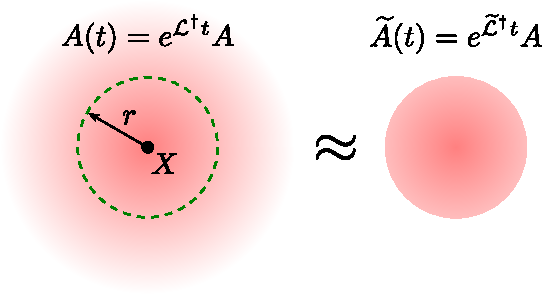
\includegraphics[scale=0.875]{figures/truncate.pdf}
  \caption{The evolution of an operator $A$ initially supported on $X$ by an adjoint Liouvillian $\L^\dag$ can be approximated by the same operator evolved by the truncated version of the Liouvillian, $\td \L^\dag$, supported on a ball of radius $r$ around $X$, up to an error given by $C(r,t)$.}
  \label{fig:LRbound_truncated}
\end{figure}

\begin{lemma}
[Bounds on the error incurred by approximating of time-evolved operators by local ones]
\label{lemma:LRbound_truncated}
    Let $A$ be an operator initially supported on a site $X\in\Lam$ and let $\td \L$ be the restriction of the long-range Liouvillian $\L$ to the ball of radius $r$ centered on $X$.
    Let $\tilde A(t)$ be the time-evolved version of $A$ under $\td \L^\dag$.
    Then the error in the approximation of $A(t)$ by $\tilde A(t)$ is bounded by
    \begin{align}
    \label{eq:LR-bound-approx}
        \|A(t) - \tilde A(t) \| \le K \|A\|\,\mathcal C(r,t),
    \end{align}
    where $K$ is some constant, and $\mathcal C(r,t)$ is a modified version of the standard Lieb-Robinson bound adapted to the problem of locally approximating time-evolved operators.
    In the large-$r$ limit, the tightest-known bounds for open systems with long-range interactions with $\alpha > d$ scale asymptotically as
    \begin{equation}
      \label{eq:LR-bound-cc}
      \ds
      \mathcal C(r,t) \propto \begin{cases} \ds
            e^{vt}/r^{\al-d},& \al > d,
        \\
        \ds t^{\alpha-d+1}/r^{\alpha-3d}
        , & \al > 3d,
        \\ \ds t^2/r^{\alpha-3},& \al > 3, d=1.
      \end{cases}
    \end{equation}
    For $\al \le d$, the bounds also depend on the system size of the lattice $N\coloneqq|\Lam|$.
    When $r \propto N^{1/d}$, the bounds scale as follows:
    \begin{equation}
      \label{eq:LR-bound-cc-small-alpha}
      \mathcal C(N,t) \propto \begin{cases}
        \ds\frac{e^{\Th{N^{1-\al/d}}t}-1}{\Th{N^{1-\al/d}}},& \al < d,
        \\
        \ds\frac{e^{\Th{\log(N)}t}-1}{\Th{\log(N)}},& \al= d.
      \end{cases}
    \end{equation}
    This concludes the statement of \cref{lemma:LRbound_truncated}.
\end{lemma}
The proof of \cref{lemma:LRbound_truncated} follows straightforwardly from the open-system Lieb-Robinson bounds detailed in \cref{sec:open-LR}.
In particular, the three lines of \cref{eq:LR-bound-cc} follow from \cref{eq:LR-ZX-open}, \cref{eq:LR-Minh-constX}, and \cref{eq:chen-lucas-open-bound}, respectively,
while \cref{eq:LR-bound-cc-small-alpha} comes from \cref{eq:LR-ZX-open-small-alpha}.
In \cref{app:sim-local-obs}, we provide the details of the derivation of the bounds in \cref{lemma:LRbound_truncated}.
We now proceed to derive the bounds on clustering of correlations in the steady states of gapped, reversible Liouvillians.

\subsection{Bound on covariance correlations}
In this first section, we show how open-system Lieb-Robinson bounds constrain the correlations in the steady state of a Liouvillian $\L$ with dissipative gap $\lambda$.

The dissipative gap $\lambda >0$
is defined as the magnitude of the least-negative non-zero real part of an eigenvalue of $\L$.
(Throughout this work, we shall also assume that the Liouvillian is \textit{primitive}, i.e.~it has a unique steady state such that $\L$ has one eigenvalue of zero.)
In addition to the Lieb-Robinson bounds,  we will also appeal to certain ``mixing bounds'' which  describe how fast  arbitrary initial states (or various correlation functions) converge to the steady state.

For the mixing bounds, we need to impose ``reversibility'' on the Liouvillian. We say that a Liouvillian $\L$ is $s$-reversible if there exists some operator $\sigma$ such that $\Gamma_s \L^\dag = \L \Gamma_s$ is satisfied;  the superoperator $\Gamma_s$ is defined via $\Gamma_s(f) = ( \sigma^s f \sigma^{1-s} + \sigma^{1-s} f \sigma^s)/2$ and $s \in[0,1]$. For $s$-reversible Liouvillians, it is easy to see that $\sigma$ is the steady state of $\L$ (since $\L^\dag (\mathbb{I}) = 0$).
A sufficient condition for a Liouvillian to satisfy $s$-reversibility (for all $s$) is if the dissipators  $L_i$ satisfy a detailed-balance condition (and the Hamiltonian is zero, $H=0$), which is naturally obeyed for systems coupled to a thermal bath \cite{Kastoryano2013}. (More explicitly, the detailed-balance condition is satisfied if dissipators come in energy raising/lowering pairs with respect to some effective Hamiltonian $\bar{H}$---for example, if $[\bar{H}, L_{\pm}] = \pm \omega L_{\pm}$ and $|L_-| / |L_+| = \exp(2 \beta \omega)$ where $\beta^{-1}$ is an effective temperature.)

Returning to the topic of correlations, we let $\rho$ be a quantum state defined on the lattice $\Lambda$.
We are interested in the \emph{covariance correlation} between non-overlapping $X,Y \in \Lambda$:
\begin{align}
\label{eq:covcorrdef}
  T_\rho (X:Y) := \text{sup}_{\norm{f} = \norm{g} = 1}|\text{Tr}[(f \otimes g)(\rho_{XY} - \rho_X \otimes \rho_Y) ] |,
\end{align}
where $f$ and $g$ are Hermitian operators with $f$ supported on region $X$ and $g$ supported on region $Y$, and where $\rho_{X}$ is the reduced density matrix constructed from $\rho$ by tracing over the complement of $X$. Our goal is to bound this correlation function in terms of $\lam$ and the distance between $X$ and $Y$.

We follow Theorem 9 in Ref.~\cite{Kastoryano2013}.
Let $\sigma$ be the steady state of the Liouvillian.
From the right-hand side of \cref{eq:covcorrdef}, we define
\begin{equation}
\text{Cov}_\sigma(  f, g) \coloneqq \frac{1}{2} \text{Tr}[(f g + g f) \sigma] -\text{Tr}[f \sigma] \text{Tr}[g \sigma],
\end{equation}
which is equivalent to the term inside the sup (because $f$ and $g$ commute).
Now we use the bound (which follows directly from the triangle inequality)
\begin{equation}
\label{eq:covcorr}
  |\text{Cov}_\sigma(f, g)| \leq |\text{Cov}_\sigma (f_t, g_t)| + |\text{Cov}_\sigma(f, g)  - \text{Cov}_\sigma(f_t, g_t)|.
\end{equation}
Here $f_t$ and $g_t$ are the time-evolved versions of $f$ and $g$ under $\L^\dag$.
This step allows us to relate a \textit{static} covariance to  time-dependent quantities;  we will use dynamical bounds to  constrain the form of the latter, then pick an optimal time which maximally bounds the static covariance.

The first term on the right is constrained by the variance bound for $s$-reversible, primitive Liouvillians (see Appendix \ref{sec:var-bound})
\begin{equation} \label{eq:cov-bound}
|\text{Cov}_\sigma (f_t, g_t)| \leq 4 \norm{f} \norm{g}  e^{-2 \lambda t},
\end{equation}
where $\lambda$ is the dissipative gap of $\L$.
Intuitively, this relationship can be understood as follows: the operators $f_t, g_t$  both evolve (in time) toward an operator  that is proportional to the identity, so the covariance between them will eventually tend to zero as a function of time. The rate at which this occurs is set by the dissipative gap of the system.

To bound the second term, we use the relation $\Tr[\sigma f_t]=\Tr[\sigma f]$, which holds for all observables $f$.
This gives:
\begin{align}
& |\text{Cov}_\sigma(f, g)  - \text{Cov}_\sigma(f_t, g_t)| \\
& = \frac12 (|\Tr[(fg-f_tg_t)\sigma] + \Tr[(gf-g_tf_t)\sigma]|) \\
& = \frac12 (|\Tr[((fg)_t-f_tg_t)\sigma] + \Tr[((gf)_t-g_tf_t)\sigma]|) \\
& \leq \frac12 (\|(fg)_t-f_tg_t\|+\|(gf)_t -g_tf_t\|) \\
& \le K \norm{f}  \norm{g} \mathcal{C}(r, t), \label{eq:secondterm}
\end{align}
where $r \coloneqq d(X,Y)$.  We obtain the inequality in the final line using the open-system Lieb-Robinson bounds $\mathcal C(r,t)$ given in \cref{lemma:LRbound_truncated}.
Specifically, we use the following Lemma, which is itself a restatement of Corollary 7 in Ref.~\cite{Kastoryano2013}:
\begin{lemma}
[Time-evolution of spatially separated observables]
  \label{lemma:connectedcorrs}
    Take two operators $A$ and $B$ supported on $X,Y \in \Lam$  respectively such that $r\coloneqq d(X,Y)$, and let $A(t)=e^{\L^\dag t}A$ and $B(t) = e^{\L^\dag t}B$ be their time-evolution under the adjoint Liouvillian $\L^\dag$.
    We also define $(AB)(t) = e^{\L^\dag t}(AB)$.
    Then the following bound holds:
    \begin{align}
    \label{eq:ops-evolving-together}
        \|(AB)(t) - A(t)B(t)\| \le K\|A\|\|B\|\mathcal C(r,t),
    \end{align}
    where $\mathcal C(r,t)$ is given by \cref{lemma:LRbound_truncated} and $K$ is some constant that depends on lattice parameters.
\end{lemma}
\cref{lemma:connectedcorrs} bounds the difference between operators that evolve together in the Heisenberg picture as opposed to evolving separately.
Again we emphasize that $A(t)$, $B(t)$, and $(AB)(t)$ are \textit{not} equivalent to Heisenberg-Langevin evolution, a fact that is at the core of this bound.
We defer the short proof of \cref{lemma:connectedcorrs} to \cref{app:connectedcorrs} and move on to proving the bound on the covariance correlations.

\begin{theorem}[Bounds on steady-state covariance correlations]
\label{theorem:covariancebound}
Consider Hermitian operators $f,g$ which are supported on two non-overlapping subsets $X$ and $Y$ of the $d$-dimensional cubic lattice $\Lambda$, and let $\L$ be an $s$-reversible Liouvillian with stationary state $\sigma$ and dissipative gap $\lambda$ that satisfies the conditions in \cref{eq:L-norm-bound}.
Then there exists a constant $c > 0$ which only depends on $\lambda, v$  such that
\begin{equation}
\label{eq:bounds-covar-correl}
T_\sigma (X:Y) \leq \begin{cases}
     \ds  c \left( r^{\alpha - d} \right)^{\frac{-2 \lambda}{ v + 2\lambda}},& \al > d,
    \\ \ds c \frac{\log(r)^{\al-d+1}}{r^{\al-3d}},& \al > 3d,
    \\ \ds c\frac{\log(r)^2}{r^{\al-3}},& \al> 3, d=1.
    \end{cases}
\end{equation}
\end{theorem}

\begin{proof}
From our previous analysis [see Eqs.~(\ref{eq:cov-bound}) and (\ref{eq:secondterm})] on the covariance correlation in \cref{eq:covcorr}, we have
\begin{equation}
|\text{Cov}_\sigma (f, g)| \leq 4 \norm{f} \norm{g}  \left(e^{-2 \lambda t} + \frac K4 \mathcal{C}(r, t) \right).
\end{equation}
To obtain the tightest bound, we  minimize with respect to $t$ the function
\begin{equation}
\label{eq:cov_corr_minimization}
h(t) =   e^{-\lambda' t} + K' \mathcal{C}(r, t),
\end{equation}
where $\lambda' = 2\lambda, K'= K/4$.

We will perform this minimization exactly for the first case in \cref{eq:bounds-covar-correl}, for which $\mathcal{C}(r,t)$ is given by the first line of \cref{eq:LR-bound-cc}; for the other cases, we instead use an approximation to the optimal ansatz, which allows us to obtain an analytical expression for the bound.
Setting $dh/dt=0$ in \cref{eq:cov_corr_minimization} leads to a minimum at time
\begin{equation}
\bar{t} = -\left( \frac{1}{\lambda'+v} \right) \log \left(  \frac{ K' v }{ \lambda r^{\alpha-d}} \right).
\end{equation}
This implies a minimum:
\begin{align}
h(\bar{t}) &= \left( \frac{K' v}{\lambda' r^{\alpha - d}} \right)^{\frac{\lambda'}{ \lambda' + v}} + \frac{K'}{r^{\alpha - d}}  \left( \frac{K' v} {\lambda' r^{\alpha - d}} \right)^{\frac{-v }{ \lambda' + v }} \nonumber \\
&\leq  c  \left( r^{\alpha - d} \right)^{\frac{-2 \lambda}{ v + 2\lambda}}
\end{align}
for some constant $c$ which depends on $\lambda, v, K$.
Taking the supremum over $f,g$ gives the bound on $T_\sigma (X:Y) $ for $\alpha > d$ in the first line of Eq.~(\ref{eq:bounds-covar-correl}).

For the other two cases, we use the ansatz $t^* = 1+\log(r^\beta)$.
Since the bound in the second line of \cref{eq:LR-bound-cc} scales as
$ \mathcal C(r,t) \propto t^{\alpha-d+1}/r^{\alpha-3d}$
for all $t$, we have
\begin{align}
  h(t^*) &= e^{-\lambda(1+\log(r^\beta))} + K \frac{(1+\log(r^\beta))^{\al-d+1}}{r^{\al-3d}}\nonumber \\
  &= \frac{e^{-\lambda}}{ r^{\lambda\beta}}+ K \frac{(\beta\log(r))^{\al-d+1}}{r^{\al-3d}}
  + \O{\frac{\log^{\al-d}(r)}{r^{\al-3d}}}.
\end{align}
We choose $\beta = (\al-3d)/\lambda$, which is positive for $\al>3d$.
This gives the ultimate bound of
\begin{align}
  h(t^*) &=  \frac{e^{-\lambda}+ K  \left( \frac{\alpha -3d}{\lambda} \log r \right)^{\alpha-d+1}}{r^{\alpha - 3d}} + \O{\frac{\log^{\al-d}(r)}{r^{\al-3d}}}\nonumber\\
  &=
   K\left(\frac{\al-3d}{\lambda}\right)^{\al-d+1}\frac{\log^{\al-d+1}(r)}{r^{\al-3d}} \nonumber\\&\quad \qquad + \O{\frac{\log^{\al-d}(r)}{r^{\al-3d}}},
\end{align}
which proves the second line of Eq.~(\ref{eq:bounds-covar-correl}). For the $d=1$ case in the last line of Eq.~(\ref{eq:bounds-covar-correl}), the argument proceeds similarly, but we obtain a slightly better scaling in the logarithmic factor.
\end{proof}

Here we discuss the scaling of the bounds in \cref{eq:bounds-covar-correl}, which is depicted in \cref{fig:light-cone-scalings}.
The effective exponent of the $1/r$-scaling of the bound for $\al > d$ is $ \al' \equiv (\alpha - d)\frac{2\lambda}{ v + 2\lambda}$, as compared to $\tilde \al \equiv \al-3$ for $\al > 3d$ (neglecting terms doubly logarithmic in $r$).
Since $\al'$ decreases as a function of $v$, the former bound becomes looser for larger $v$.
In more detail, if we let $x = \frac v\lambda$, then $\al' < \tilde \al$ for all $\al > \frac{(3x+4)d}{x}$.
In the limit of $x\ra \infty$, $\tilde \al$ is tighter for all $\al > 3d$.
Thus, for large enough $\al$ and $v$, the power-law light-cone bounds [second line in Eq.~(\ref{eq:LR-bound-cc}), which in turn comes from Eq.~(\ref{eq:LR-Minh-constX})]  give asymptotically tighter bounds on the clustering of covariance correlations than the logarithmic light-cone bound [first line in Eq.~(\ref{eq:LR-bound-cc}), which in turn comes from Eq.~(\ref{eq:LR-ZX-open})].

\begin{figure}[h]
\centering
\label{fig:model1}
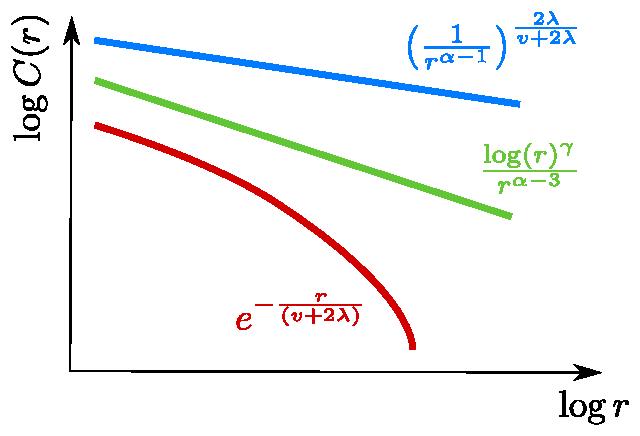
\includegraphics[width=.45\textwidth]{figures/light-cones-log.pdf}
\caption{A log-log plot of the tails of the bounds on the various connected correlation functions in Theorems 1, 2, and 3 for $d = 1$. We include the exponentially decaying tail from the short-range interactions case (red curve) for comparison.
For the power-law decaying bounds, we have different scaling exponents of the power-law tails for the bound for $\alpha >1$ (blue curve) and the bound for $\alpha > 3$ (green curve).
For a given choice of $x = \frac v\lambda$, the relative positioning of the curves
holds for all $\al > \frac{3x+4}{x}$.
In the limit $v \gg \lambda$, the picture holds for all $\al > 3$.}
  \label{fig:light-cone-scalings}
\end{figure}

\subsection{Stability result and mutual information bound}
In this section, we will  use the aforementioned bounds to constrain steady-state properties of open systems with power-law interactions.
In addition to the newly-derived Lieb-Robinson bounds,  we will  appeal to a ``mixing bound'' which provides an upper bound to how fast an arbitrary initial state will converge to the steady state. The following mixing bound was derived in Ref.~\cite{Kastoryano2013d}, and generalizes the mixing bound of classical Markov chains to quantum semigroups:

\begin{lemma}
  \label{cor:mixing}
    Consider a  primitive Liouvillian $\L$ that has a  full-rank steady state  $\sigma$, and is $\frac12$-reversible. Then an arbitrary initial state $\rho$ will converge to $\sigma$ at a rate bounded by
    \begin{equation}
        \lVert \rho(t) - \sigma \lVert_1 \leq \sqrt{2 \log( \lVert \sigma^{-1} \lVert )} e^{-\beta t},
    \end{equation}
    where $\beta$ is called the log-Sobolev constant associated with $\L$.
\end{lemma}
Intuition can be gained by considering an  ``infinite-temperature'' steady state $\sigma = \mathbb{I} /
d_{H}$ where $ d_{H}$ is the dimension of the Hilbert space.  The mixing bound above states that the coefficient in front of the exponential will  scale as $\sqrt{\log(d_{H})}$, i.e.~it will increase with the dimension of the Hilbert space. This is because the convergence toward the unique steady state from an arbitrary initial state can be slow if the dimension of the Hilbert space is large.


\begin{theorem}[Effect of perturbations on reduced steady-state density matrix]
\label{thm:stability_results}
Let $X,Y$ be two non-overlapping subsets of a $d$-dimensional cubic lattice $\Lambda$.  Let $\L_1 $  be a primitive and $\frac12$-reversible Liouvillian with log-Sobolev constant $\beta$, and let $\L_2$ be a Liouvillian perturbation, acting trivially outside of $X$. Let $\rho$ be the stationary state of $\L_1$, and let $\sigma$ be the stationary state of $\L_1  + \L_2$. Then,
\begin{equation}
\label{eq:perturbation_bounds}
\lVert \rho_Y - \sigma_Y  \lVert_1 \leq
\begin{cases}
    \ds c \log (  \lVert \rho^{-1}  \lVert)^{\frac12} \left(\frac1{r^{\alpha - d}} \right)^{\frac{2 \beta}{ v + 2\beta}},& \al > d,
    \\ \ds c \log (  \lVert \rho^{-1}  \lVert)^{\frac12} \frac{\log(r)^{\al-d+1}}{r^{\al-3d}},& \al > 3d,
    \\ \ds c \log (  \lVert \rho^{-1}  \lVert)^{\frac12} \frac{\log(r)^2}{r^{\al-3}},& \hspace{-2em}\al> 3, d=1,
\end{cases}
\end{equation}
where $c$ is a constant and $r$ is the distance between $X$ and $Y$.
\end{theorem}

The theorem basically says that the effects of local perturbations in the Liouvillian will not be felt significantly by the steady state of the system at sufficiently distant locations.
We prove the theorem by first introducing a time-evolved state to interpolate between the two steady states.
This allows us to use a combination of mixing-time and Lieb-Robinson bounds to restrict the terms in this bound.
Then we apply the same minimization procedure used in \cref{theorem:covariancebound} for the covariance-correlations bound to arrive at the stated bounds in \cref{eq:perturbation_bounds} [each of which follow directly from the three cases in \cref{eq:LR-bound-cc}].
We defer the proof of this result, which is similar to the proof of \cref{theorem:covariancebound}, to \cref{app:proof-stability}.

We now prove a bound on the mutual information in the steady state.  The mutual information between two regions $A,B$ is defined as
\begin{equation}
I_\rho(A:B) = S(\rho_{AB} || \rho_A \otimes \rho_B),
\end{equation}
where $S(\rho || \sigma )= \tr[\rho ( \log \rho - \log \sigma)]$ is the relative entropy. The following theorem holds.

\begin{theorem} [Clustering of mutual information]
\label{thm:mutual_information_clustering}
Let $A,B$ be two non-overlapping subsets of a $d$-dimensional cubic lattice $\Lambda$.  Let $\L $  be a primitive and $\frac12$-reversible Liouvillian with log-Sobolev constant $\beta$. Let $\rho$ be the stationary state of $\L$. Then the mutual information between the two regions $I_\rho(A:B)$ is bounded by
\begin{equation}
I_\rho(A:B)  \leq \begin{cases}
       \ds c \log (  \lVert \rho^{-1}  \lVert)^{\frac32} \left( \frac1{r^{\alpha - d}} \right)^{\frac{2 \beta}{ v + 2\beta}},& \al > d,
    \\ \ds  c \log (  \lVert \rho^{-1}  \lVert)^{\frac32} \frac{\log(r)^{\al-d+1}}{r^{\al-3d}},& \al > 3d,
    \\ \ds c\log (  \lVert \rho^{-1}  \lVert)^{\frac32} \frac{\log(r)^2}{r^{\al-3}},& \hspace{-2em}\al> 3, d=1,
    \end{cases}
\end{equation}
where $c$ is a constant and $r$ is the distance between $A,B$.
\end{theorem}

The significance of this result is that the mutual-information correlations in the steady state of an open long-range system decay as a power-law in the distance between regions.
This bound, which relies on the existence of the log-Sobolev constant, is tighter than the naive bound that would result from simply applying the bound on the covariance correlation in \cref{theorem:covariancebound} to $I_\rho(A:B)$.

\begin{proof}

We define the semi-group $\tilde{\L}$ to be the terms in $\L$ that act entirely within balls of radius $r/2$ centered around $A$ and $B$, and let $\sigma$ be the steady state of  $\tilde{\L}$. Simple manipulations imply:
\begin{align}
I_\rho(A:B) &= - S(\rho_{AB})  + S(\rho_A)  + S(\rho_B) \\
& \leq  - S(\rho_{AB})  - \tr[ \rho_A \log \sigma_A ] -  \tr[ \rho_B \log \sigma_B ] \\
&=  S(\rho_{AB} || \sigma_A \otimes \sigma_B).
\end{align}
where we have used $S(\rho || \sigma) \geq 0$ to obtain the inequality.
The RHS further  satisfies the inequality:
\begin{equation}
S(\rho_{AB} || \sigma_A \otimes \sigma_B) \leq \log( ||\rho_{AB}^{-1} ||) || \rho_{AB} - \sigma_A \otimes \sigma_B ||_1,
\end{equation}
which is a standard result (c.f. Eq.~(36) in Ref.~\cite{Kastoryano2013}).
From here, we can apply the bounds in \cref{thm:stability_results}, using $\L_1 = \td \L $, $\L_2 = \L - \td \L$, $Y = A\cup B$, and $X = \Lambda \setminus Y$.
\end{proof}

\section{Summary and outlook}

In this work, we have proven generalized Lieb-Robinson bounds which constrain the dynamics of open, Markovian systems with power-law interactions and used them to constrain correlations in the steady state.

We comment briefly on the tightness of the bounds derived in this work. Intuitively, one might expect that the presence of dissipation should lead to tighter Lieb-Robinson bounds for open systems than for their closed counterparts, since the presence of decoherence from a bath might  limit the speed of quantum information transfer.
In this work, we have  generalized the proof of Lieb-Robinson bounds from closed system dynamics to Markovian evolution (\textit{a priori}, such bounds need not exist for Markovian dynamics).
However, our bounds only depend on interaction range and the dimension of the lattice.
Any bound that only depends on these two inputs cannot be tighter than the corresponding closed-system Lieb-Robinson bound, since the latter is a special case of former.
As such, the saturating protocols for closed systems \cite{Tran2020hierarchylinearlightcones,Tran2021} can be used to saturate open Lieb-Robinson bounds such as those uncovered in  \cref{lemma:LRbound_truncated}.
In the future, it would be interesting to add another degree of freedom into formulations of open Lieb-Robinson bounds: the dissipative gap. (Some progress has been made in showing that Lieb-Robinson velocities can get tighter in dissipative systems \cite{descamps2013}.)
In principle, it might be possible to derive Lieb-Robinson bounds that reduce to closed-system ones when the dissipative gap is zero, and get tighter in the presence of non-zero dissipation.
Then one can develop protocols that saturate the dissipative-gap-dependent bounds.
Another question in this direction is whether the conditional evolution generated via a non-Hermitian Hamiltonian can also exhibit a dissipative-gap-dependent Lieb-Robinson bound that reduces to the conventional one in the dissipationless limit.

Setting aside the idea of a Lieb-Robinson bound that depends on the dissipative gap, there is still the question of generalizing the best-known closed-system bounds to Markovian evolution. In particular, the recent Lieb-Robinson bounds in Refs.~\cite{kuwaharaStrictlyLinearLight2020} and \cite{Tran2021b} both provide opportunities for generalization to open systems.
Such a result would likely require a modification of the interaction-picture technique first developed in \cite{Foss-Feig2015} and used in both subsequent works to open-system dynamics.
Generalizing these bounds would directly lead to tighter bounds on operator spreading in \cref{lemma:LRbound_truncated} and allow us to prove tighter bounds on correlation clustering in steady states (\cref{theorem:covariancebound} and \cref{thm:mutual_information_clustering})

Another way to probe the tightness of the steady-state correlation bounds derived in this work would be to improve the mixing bounds, which currently require the open system to be in thermal equilibrium.
It would be interesting to derive more general mixing bounds which also apply to systems that are out of thermal equilibrium.

One of the salient applications of Lieb-Robinson bounds is in rigorous proofs on the  stability of  the spectral gap in topologically ordered quantum matter. For example, Ref.~\cite{Bravyi2010} used closed-system Lieb-Robinson bounds to  show that spatially local perturbations will not close energy gaps in the toric code, thus leading to phase stability against arbitrary local noise. Can we use a similar approach to show that local perturbations will not close the dissipative gap in a topologically-ordered open system? A robust qubit steady-state structure would be useful toward the quest of passive quantum error correction \cite{Lidar1998}.

Lieb-Robinson bounds can be used  to prove area-law entanglement scaling in the ground state of one-dimensional systems with local interactions \cite{Hastings2007}. This result helps to rigorously justify the validity of the matrix-product state  ansatz for the ground state of such systems.  For closed systems with power-law interactions, Lieb-Robinson bounds can be used to further extend area-law scaling to certain broad classes of systems \cite{Gong2017}. Do the results presented in this paper have similar implications for area-law scaling of the steady state? This would have direct implications for the matrix-product operator ansatz in modeling open systems.

Finally, the Lieb-Robinson-type bounds we proved apply for the operator, or $\infty$-norm.
However, there exists a hierarchy of Lieb-Robinson-like bounds that have the potential to be tighter for certain information processing tasks such as scrambling and transferring a quantum state of a local subsystem without knowledge of the initial state of the rest of the system.
These bounds can use other norms such as the Frobenius norm defined by $\|O\|_F = \sqrt{\Tr{O^\dag O}}$ \cite{Tran2020hierarchylinearlightcones,Kuwahara2020aPolynomialGrowthOutoftimeorder,Yin2020ScramblingAlltoall,Chen2021Frobenius} or apply to free-particle systems \cite{Guo2019,Tran2020hierarchylinearlightcones}.
It would be interesting to generalize these bounds to open systems as well.
 %Still has compilation errors

\chapter{Conclusion}
We conclude with some discussion of open directions.

$VLR scrambling$

Finding an optimal protocol that saturates the Lieb-Robinson bounds for $\al \le d$ is still an open question, even though we've proven that the bounds are tight for many-site signaling.
Also, recent work has shown that the scrambling time is better bounded by the so-called Frobenius bound, which has been shown to yield tighter bounds than the Lieb-Robinson bound for the Frobenius norm of the unequal-time comutator (which can be related to the out-of-time-order correlator). Indeed, a hierarchy of linear light cones has been shown in which the Frobenius bound yields a finite scrambling speed at a smaller value of $\alpha$ than the Lieb-Robinson bound does for signaling, thus clearly delineates these types of bounds \cite{Tran2020hierarchylinearlightcones}.
For higher dimensions, the conjectured Frobenius light cone is $t$\,$=$\,$\W{r^{\alpha-d}}$ for $d$\,$<$\,$\al$\,$<$\,$d+1$ \cite{Chen2021Frobenius}.
If this generalization of the Frobenius bound were to hold, our lower bounds on the circuit complexity of QFT and fanout in \cref{ch:qfo} would immediately generalize.

%QFO

We have derived our lower bounds on $t_\textrm{QFT}$ under the assumption that the first and last qubits of the QFT are separated by a distance of $r$\,$=$\,$\Theta(n^{1/d})$.
However, other mappings of computational qubits to lattice qubits could potentially lead to faster implementations.
For example, consider the mapping onto a one-dimensional chain of qubits wherein the second half of the chain is interleaved in reverse order with the first half \footnote{Specifically, for even $n$, this mapping is defined by $q_i\mapsto q_{2i-1}$ for $i \le n/2$ and $q_i\mapsto q_{2(n-i+1)}$ for $i > n/2$.}.
Applying the QFT to a product state in this layout results in a state with two-qubit correlations that decay exponentially in the distance between the qubits.
In this case, our lower bound techniques cannot rule out the possibility of $t_\textrm{QFT}$\,$=$\,$o(n)$ for short-range interacting Hamiltonians.
This suggests that $t_\textrm{QFT}$ could depend strongly on qubit placement.
Given that the QFT is typically used as a subroutine for more complex algorithms, it may not always be possible to reassign qubits without incurring costs elsewhere in the circuit.
Still, it would be interesting to investigate whether careful qubit placement could yield a faster QFT.

% OCC
In this work, we have  generalized the proof of Lieb-Robinson bounds from closed system dynamics to Markovian evolution (\textit{a priori}, such bounds need not exist for Markovian dynamics).
However, our bounds only depend on interaction range and the dimension of the lattice.
Any bound that only depends on these two inputs cannot be tighter than the corresponding closed-system Lieb-Robinson bound, since the latter is a special case of former.
As such, the saturating protocols for closed systems \cite{Tran2020hierarchylinearlightcones,Tran2021a} can be used to saturate open Lieb-Robinson bounds such as those uncovered in  \cref{lemma:LRbound_truncated}.
In the future, it would be interesting to add another degree of freedom into formulations of open Lieb-Robinson bounds: the dissipative gap. (Some progress has been made in showing that Lieb-Robinson velocities can get tighter in dissipative systems \cite{descamps2013}.)
In principle, it might be possible to derive Lieb-Robinson bounds that reduce to closed-system ones when the dissipative gap is zero, and get tighter in the presence of non-zero dissipation.
Then one can develop protocols that saturate the dissipative-gap-dependent bounds.
Another question in this direction is whether the conditional evolution generated via a non-Hermitian Hamiltonian can also exhibit a dissipative-gap-dependent Lieb-Robinson bound that reduces to the conventional one in the dissipationless limit.

Lieb-Robinson bounds can be used  to prove area-law entanglement scaling in the ground state of one-dimensional systems with local interactions \cite{Hastings2007}. This result helps to rigorously justify the validity of the matrix-product state  ansatz for the ground state of such systems.  For closed systems with power-law interactions, Lieb-Robinson bounds can be used to further extend area-law scaling to certain broad classes of systems \cite{Gong2017}. Do the results presented in this paper have similar implications for area-law scaling of the steady state? This would have direct implications for the matrix-product operator ansatz in modeling open systems.

Finally, the Lieb-Robinson-type bounds we proved apply for the operator, or $\infty$-norm.
However, there exists a hierarchy of Lieb-Robinson-like bounds that have the potential to be tighter for certain information processing tasks such as scrambling and transferring a quantum state of a local subsystem without knowledge of the initial state of the rest of the system.
These bounds can use other norms such as the Frobenius norm defined by $\|O\|_F = \sqrt{\Tr{O^\dag O}}$ \cite{Tran2020hierarchylinearlightcones,Kuwahara2020aPolynomialGrowthOutoftimeorder,Yin2020ScramblingAlltoall,Chen2021Frobenius} or apply to free-particle systems \cite{Guo2019,Tran2020hierarchylinearlightcones}.
It would be interesting to generalize these bounds to open systems as well.


\appendix

% \chapter{Supplemental Material for Chapter 1}

In \cref{sec:generalbound}, we provide a detailed proof of the general Lieb-Robinson-type bound for long-range interactions with $\al\le d$ mentioned in \cref{eq:newbound}. The bound has a closed-form expression that can be used to lower bound the signaling time [see \cref{eq:tsi}] for $\al \le d$.

In \cref{sec:exactsumbound}, we derive a second general Lieb-Robinson-type bound that is the tightest one can get from the Lieb-Robinson series mentioned in \cref{eq:HKseries1}, although it lacks a closed-form analytic expression.
We show numerically that the signaling time obtained from this bound has the same scaling as a function of system size $N$ as the bound in \cref{eq:newbound} when $N$ is sufficiently large.
Therefore, the bound presented in \cref{eq:newbound} is\dash in a broad sense\dash the best one can obtain without developing new techniques beyond those used in deriving the traditional Lieb-Robinson series.

\section{Proving the general Lieb-Robinson-type bound for \texorpdfstring{$\al \le d$}{α <= d}}
\label{sec:generalbound}
Before we present the proof of the general Lieb-Robinson-type bound given in \cref{eq:newbound}, let us summarize in \cref{sec:math} some mathematical preliminaries useful for the proof.

\subsection{Mathematical preliminaries}
\label{sec:math}
In this section, we elaborate on the scaling of the on-site hop parameter $J_{ii}$ defined after \cref{eq:hoppingterms}.
We define the quantity $\lambda = \max_{i\in\Lambda} J_{ii}$, which for power-law interactions has strength
\begin{equation}
	\label{eq:self-hop}
	\lam = \max_{i\in\Lam} \sum_{j\in\Lam\backslash i} J_{ij} = \max_{i\in\Lam}\sum_{j\in\Lam\backslash i} \frac{1}{r_{ij}^{\al}}.
\end{equation}
If the lattice $\Lam$ is a square lattice with unit spacings, then $\lambda$ scales as
\begin{equation}
        \label{eq:lamdef2}
	\lam = \begin{cases}
        \Th{N^{1-\al/d}} & \text{for }0\le\al<d,\\
        \Th{\log N} & \text{for }\al=d,\\
        \Th 1 & \text{for }\al>d.
\end{cases}
\end{equation}
In general, the scaling of $\lam$ as a function of $N$ in \cref{eq:lamdef2} holds asymptotically for large regular lattices \cite{Storch15}.

For $\al \le d$, we note that $\lam$ diverges in the thermodynamic limit.
For some applications, it is preferred to apply a normalizing factor of $1/\lam$ (due to Kac \cite{Kac63}) to the Hamiltonian to ensure the system energy is extensive. Since experimental systems (such as those with dipolar interactions in 3D) do not necessarily have extensive energy, we would prefer not to apply the Kac normalization. The light cone contours for Kac-normalized Hamiltonians follow straightforwardly from our results upon rescaling the time by a factor of $\lambda$.

In the rest of this subsection, we justify the dependence of $\lambda$ on $N$ and $\al$ as shown in \cref{eq:lamdef2}.
We assume that the lattice $\Lam$ is $d$-dimensional with $N = L^d$ sites.
Without loss of generality, let $i$ be the site located at the origin and define $r_j \equiv r_{ij} \ge 1$.
For $0\le \al < d$, we bound \cref{eq:self-hop} above by an integral:
\begin{align}
	\sum_{j\in\Lam} \frac{1}{r_{j}^{\al}} &\le \int_{\vec{r}\in \mathbb{R}^d} \frac{d^d\vec{r}}{\|\vec{r}\|^\al}
	= \frac{2\pi^{\frac d 2}}{\Gamma(\frac d2)} \int_0^L \frac{dr}{r^{\al-d+1}}  = \frac{\omega_d}{d-\al}L^{d-\al},
\end{align}
where $\omega_d\equiv 2\pi^{\frac d 2}\big/\Gamma(\frac{d}{2})$ is the hyper-surface area of a unit $d$-sphere and $\Gamma(\cdot)$ is the Gamma function.  It follows that $\lam = \O{ N^{1-\al/d}}$  for $\al<d$.
The asymptotic lower bound $\lam = \W{N^{1-\al/d}}$ follows from setting $\|\vec r\| \rightarrow \|\vec r\| +\sqrt d$ and integrating from $r=1$ to $r=\infty$.

For $\al = d$, we perform the same calculation, taking care to avoid integrating over the origin:
\begin{align}
	\sum_{j\in\Lam} \frac{1}{r_{j}^{\al}} &\le  \int_{\|\vec{r}\| \ge 1} \frac{d^d\vec{r}}{\|\vec{r}\|^d} + \sum_{j \in \Lam} \theta \left( 1+\sqrt{d} - r_j\right)
    \\ & \le  \omega_d \int_1^L \frac{dr}{r} + \frac{\omega_d\left(1+\sqrt d+\frac12\right)^d}{\omega_d\left(\frac12\right)^d}
    \\ &= \frac {\omega_d}d \log(N) + \left(2\sqrt d+3\right)^d,
\end{align}
where $\theta(\cdot)$ denotes the Heaviside step function. So, at the critical point $\al=d$, we have $\lam = \O{ \log(N)}$.
The lower bound $\lam = \W{\log(N)}$ holds in a similar fashion.

For $\al > d$, the sum in \cref{eq:self-hop} converges, so $\lam$ can be bounded by a constant independent of $N$.
Thus, we have verified the asymptotic scaling of the on-site parameter $\lam$ for the three cases listed in  \cref{eq:lamdef2}.

\subsection{Proof of the bound in \cref{eq:newbound}}
\label{sec:newbound}

In this section, we provide a simple proof of \cref{eq:newbound} for long-range interactions.
First, let us recall the Lieb-Robinson series from \cref{eq:HKseries1}.
\begin{align}
	\label{eq:HKseries2}
		\|[A(t),B]\| &\le 2\|A\|\|B\||X||Y|\sum_{k=1}^{\infty}\frac{(2t)^{k}}{k!} \J^k(X,Y), \\
	\label{eq:hopping2}
	\J^k(X,Y) &\equiv \sum_{i_{1},\dots,i_{k-1}}J_{Xi_{1}}J_{i_{1}i_{2}}\dots J_{i_{k-1}Y}.
\end{align}
We use the so-called \emph{reproducibility condition} for finite systems with power-law decaying interactions \cite{HK, Gong14}. Specifically, for $\al > 0$ and distinct $i,j\in \Lam$, the second-order hopping term $k=2$ in \cref{eq:hopping2} can be bounded by
\begin{equation}
	\label{eq:repcon}
	\J^2(i,j) = \sum_k J_{ik}J_{kj} \le p\lam J_{ij},
\end{equation}
where $p=2^{\al+1}$ and $\lam$ is the on-site hop parameter defined in \cref{eq:self-hop}.
This inequality allows the power-law decay of $J_{ij}$ to be reproduced across multiple hopping terms.

We reorder the summations on the right-hand side of \cref{eq:hopping2} by introducing a new index $n$ to count the number of self-hops in a particular sequence of hopping sites $\{i_1,\dots,i_{k-1}\}$.
Specifically, $n$ represents the number of indices $j\in\{0,\dots,k-1\}$ such that $i_{j}=i_{j+1}$ (with $i_{0}=X$ and $i_{k}=Y$).
Now let us first assume that the $n$ self-hops occur in the first $n$ terms ($J_{Xi_1}$ to $J_{i_{n-1}i_{n}}$). Then we may rewrite the right-hand side of \cref{eq:hopping2} as
%
\begin{equation}
\label{eq:selfhopresum}
\sum_{i_{1},\dots,i_{k-1}}J_{Xi_{1}}\dots J_{i_{k-1}Y}
= \lambda^n \sum_{i_{n+1},\dots,i_{k-1}}J_{i_{n}i_{n+1}}\dots J_{i_{k-1}Y},
\end{equation}
%
using the fact that each self-hop term $J_{ii}$ is equal to $\lam$.
If, on the other hand, the $n$ self-hops appear in arbitrary positions in the sequence of hops, then accounting for these cases multiplies \cref{eq:selfhopresum} by the combinatorial factor of $\binom k n$.
Inserting into \cref{eq:hopping2} gives
%
\begin{align}
	\label{eq:choose}
	\J^k(X,Y) = \sum_{n=0}^{k}{\binom k n}\lambda^{n} \left[\sum_{i_{n+1},\dots,i_{k-1}}J_{i_Xi_{n+1}}\dots J_{i_{k-1}Y} \right],
\end{align}
where we relabeled $i_n$ as $X$.
Now, using the fact that $i_{j}\neq i_{j+1}$ for $j=n,\dots,k-1$ (where $i_k=Y$), we can apply the reproducibility condition in \cref{eq:repcon} a total of $k-n$ times along with the normalization condition $J_{ij} = 1/r_{ij}^{\al}$ for $i\neq j$ to get
%
\begin{align}
	\sum_{i_{n+1},\dots,i_{k-1}}J_{Xi_{n+1}}\dots J_{i_{k-1}Y} \le (\lam p)^{k-n-1} J_{XY} = \frac{(\lam p)^{k-n-1}}{r_{XY}^{\al}}.
\end{align}
%
Finally, inserting this inequality into \cref{eq:choose} and applying the binomial theorem gives
\begin{equation}
\mathcal{J}^{k}(r_{XY}) \le \sum_{n=0}^{k}{\binom k n}\lambda^{n}\left[\frac{(\lambda p)^{k-n-1}}{r_{XY}^{\al}}\right]\ = \frac{(\lambda+\lambda p)^{k}}{\lambda pr_{XY}^{\al}}.
\end{equation}
Inserting this bound for $\mathcal{J}^{k}(r_{XY})$ into \cref{eq:HKseries2} gives an exponential series bound for the commutator
\begin{align}
	\|[A(t),B]\| &\le 2\|A\|\|B\||X||Y|\sum_{k=1}^{\infty}\frac{(2t)^{k}}{k!} \J^k(X,Y) \\
    &\le 2\|A\|\|B\||X||Y|\sum_{k=1}^{\infty}\frac{(2t)^{k}}{k!} \frac{(\lambda(1+p))^{k}}{\lambda pr_{XY}^{\al}}\\
    &= 2\|A\|\|B\||X||Y| \left(\frac{e^{2\lam t(1+p)}-1}{\lambda pr_{XY}^{\al}}\right) \\
    &= 2\|A\|\|B\||X||Y|\left(\frac{e^{\Theta(N^{1-\al/d})t}-1}{\Theta(N^{1-\al/d})r_{XY}^\al}\right), \label{eq:newbound2}
\end{align}
which reproduces \cref{eq:newbound}.


\section{Second general Lieb-Robinson-type bound for \texorpdfstring{$\al \le d$}{α <= d}}
\label{sec:exactsumbound}
The above derivation of the bound in \cref{eq:newbound2} requires the use of the reproducibility condition~[\cref{eq:repcon}], which can make the bound loose compared to the Lieb-Robinson series in \cref{eq:HKseries2}. In this section, we will exactly sum the series in \cref{eq:HKseries2} and compare the resulting bound to that of \cref{eq:newbound2}. We will show by numerical analysis that\dash although the bound obtained directly from the Lieb-Robinson series is tighter than the one \cref{eq:newbound2}\dash it largely shares the same scaling behavior when the number of sites $N$ is large.

\subsection{Summing the Lieb-Robinson series exactly}
\label{sec:exactsumboundproof}
We now exactly calculate the sum in \cref{eq:HKseries2} without using the reproducibility condition. Since \cref{eq:HKseries2} is an infinite series, one cannot perform the sum directly. But using a discrete Fourier transform, the series can be summed numerically in a highly efficient manner.

To use the discrete Fourier transform, we assume that $J_{ij}=1/r_{ij}^\al$ is translationally invariant. Note that the physical interaction strength between lattice sites does not need to be translationally invariant, as it just needs to be bounded by $J_{ij}$. his additional assumption does not greatly affect the generality of the following results.

For simplicity, we consider a 1D lattice $\Lam$ that consists of $N$ spins on a ring; the following results generalize straightforwardly to lattices in arbitrary dimensions. Let $r_{ij} = \min\{|i-j|,|N-i+j|\}$ be the (periodic) distance metric, which coincides with the graph distance $d(i,j)$ on $\Lam$. Due to translational invariance, we denote $J_{ij}$ by $J(r_{ij})$ which satisfies $J(r+N) = J(r)$.

We now perform a discrete Fourier transform from the position space parameterized by $r=0,1,2,\cdots,N-1$ to a momentum space parameterized by $p=0,1,2,\cdots,N-1$, denoted by $\mathcal{F}_p[f(r)]=\sum_{r=0}^{N-1}e^{-2\pi ipr/N}f(r)$.
We observe that the sum in the definition of $\J^k(X,Y)$ in \cref{eq:hopping2} can be rewritten as the $k$-fold convolution of $J(r)$ with itself.
Thus, letting $r\equiv r_{XY}$ and $\J^k(r) \equiv J^k(X,Y)$, the discrete Fourier transform of \cref{eq:hopping2} is given by
\begin{align}
	\mathcal{F}_p[\J^{k}(r)]  = \omega(p)^k,
\end{align}
where $\omega(p)=\mathcal{F}_p[J(r)]$.
We now take the discrete Fourier transform of the entire series in \cref{eq:HKseries2}:
\begin{align}
\mathcal{F}_p\left[	\|[A(t),B]\|\right] & \le\sum_{k=1}^{\infty}\frac{(2t)^{k}}{k!}\omega(p)^k = e^{2\omega(p)t}-1. \label{eq:fcomm}
\end{align}
The series in \cref{eq:HKseries2} can thus be evaluated exactly by taking the inverse Fourier transform of \cref{eq:fcomm}:
%
\begin{equation}
	\label{eq:exactbound}
		\|[A(t),B]\| \le \mathcal{F}_r^{-1}\left[e^{2\omega(p) t}-1\right].
\end{equation}
where $\mathcal{F}_r^{-1}[g(p)]\equiv\frac{1}{N}\sum_{p=0}^{N-1}e^{2\pi ipr/N}g(p)$ defines the inverse discrete Fourier transform.
For $\al = 0$, the inverse Fourier transform can be evaluated to yield the analytical expression \begin{equation}
    \|[A(t),B]\| \leq 2\|A\|\|B\||X||Y|\left(\frac{e^{4Nt}-1}{N}\right),
\end{equation}
which matches the bound in \cref{eq:newbound2} up to constant factors.
For $\al > 0$, it is difficult to obtain a simple analytical expression for the bound in \cref{eq:exactbound}. We will thus evaluate this bound numerically, as detailed in the next section.

\subsection{Numerical comparison of the two bounds}
\label{exactboundnumerics}

In this section, we study the asymptotic scaling of the exact summation bound in \cref{eq:exactbound}.
Because the discrete Fourier transform can be performed rather efficiently using the Fast Fourier Transform algorithm \cite{FFT65} numerically, we can evaluate the right-hand side of \cref{eq:exactbound} for system sizes up to the order of $10^6$.
This allows us to compare the bound in \cref{eq:exactbound} (referred to below as the ``exact summation bound") with the bound in \cref{eq:newbound2} (referred to below as the ``analytical bound") for large $N$.

Let us first focus on the large-$r$ asymptotic behavior of the two bounds.
As a typical example, we set $N = 10^6$ and $t = 1/\lam$ and plot the right-hand side of the two bounds (with $\|A\|=\|B\|=|X|=|Y|=1$) as a function of $r$ for $\al = 0.5$ in \cref{Fig_Rdep}.
Unsurprisingly, the right-hand side of the analytic bound in \cref{eq:newbound2} decays as $1/r^{\al}$ for the entire range of $r$.
The exact summation bound leads to the same scaling for small $r$, but not for large $r$.
While this comparison leaves room for potential tightening of the bound in \cref{eq:newbound2} for large $r$, generic improvement of the bound for all $r$ seems unlikely.

\begin{figure}[h]
\centering
	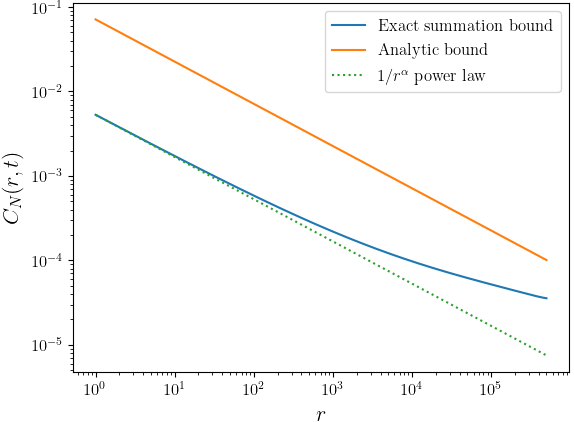
\includegraphics[width=.5\linewidth]{figures/Rdep.png}
    \caption{A comparison between the exact summation bound [\cref{eq:exactbound}] and the analytical bound [\cref{eq:newbound2}] sites as a function of the distance $r$ between operators $A$ and $B$. The specific plot assumes a 1D periodic lattice with $N = 10^6$, $\al = 0.5$, $t = 1/\lam$, and $r=1,2,\cdots,N/2$.}
    \label{Fig_Rdep}
\end{figure}

Next, we compare the $N$-dependence of the two bounds. To get rid of the $r$-dependence, we will compare the signaling times between two sites with either $r=1$ (the smallest possible separation on a 1D ring) or $r=N/2$ (the largest possible separation).
If the two bounds agree with each other at both $r=1$ and $r=N/2$ in the large $N$ limit, it is reasonable to believe that they will agree with each other at all values of $r$.

For $\al < 1$, the analytical bound gives the following signaling time (upon setting $\|[A(t),B]\|= 1$) as function of $r$ and $N$:
\begin{equation}
	\label{eq:contour_al<d}
	t_\text{si}(r,N) =\W{\frac{\log(N^{1-\al}r^{\al})}{N^{1-\al}}}.
\end{equation}
Choosing either $r=1$ or $r=N$ leads to $t_\text{si}=\Omega(N^{\al-1}\log(N))$, consistent with \cref{eq:tsi}. For the exact summation bound, we numerically compute $t_\text{si}$ by finding the value of $t$ that makes $\|[A(t),B]\| = 1$ over a range of $N$ from $10^4$ to $10^6$ for both $r = 1$ and $r = N/2$. We then fit $t$ as a function of $N$ to the function $a N^\gamma \log(N)$.
\begin{figure*}[h]
	\subfigure[~$r = 1$]{
	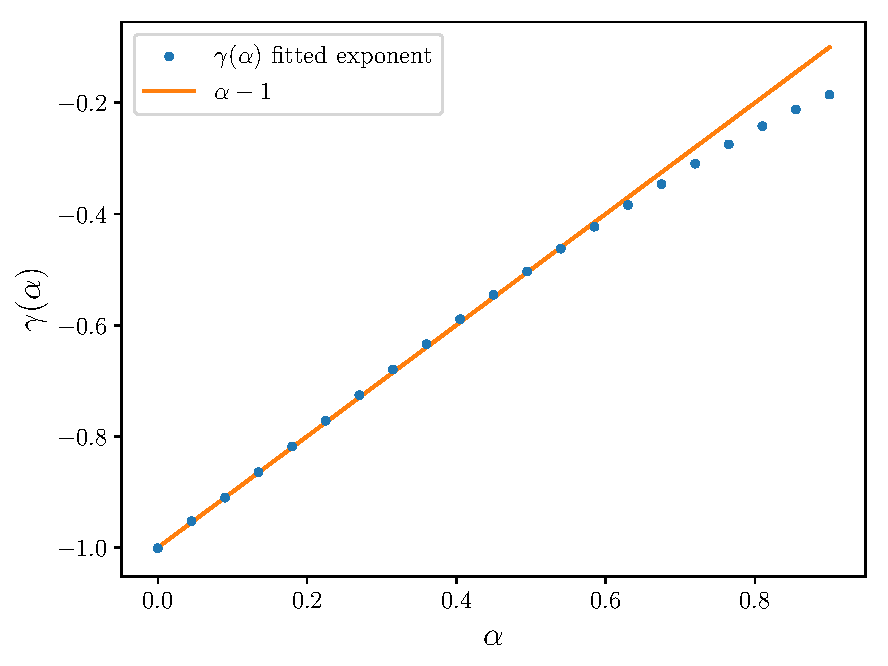
\includegraphics[width=.45\textwidth]{figures/beta_0.pdf}
    } \qquad
    \subfigure[~$r = N/2$]{
    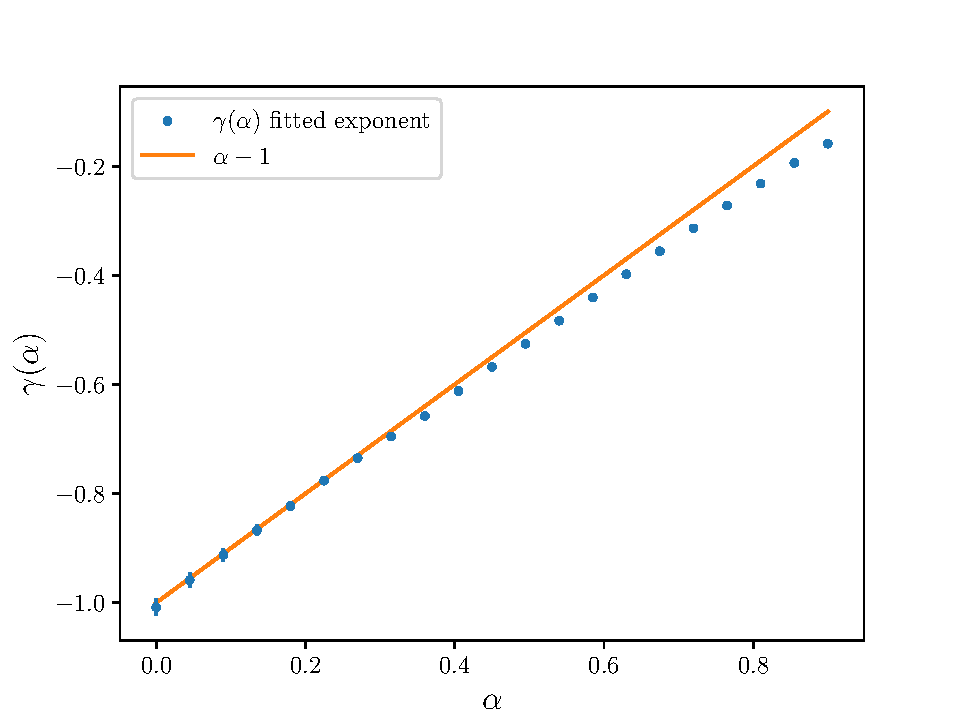
\includegraphics[width=.455\textwidth]{figures/beta_1.pdf}}
	\caption{The fitted exponent $\gamma$ in the signaling time scaling obtained from the exact summation bound in \cref{eq:exactbound} at $r=1$ (a) and $r=N/2$ (b) for $a\in [0,1]$. The error bars reflect the 95\% confidence intervals for the fit.}
        \label{Fig_al<d}
\end{figure*}
In \cref{Fig_al<d}, we plot the fitted exponent $\gamma(\al)$ as a function of $\al$. We observe that $\gamma(\al)$ scales approximately as $\al-1$ as long as $\al$ is not close to 1 for both $r=1$ and $r=N$, showing that both bounds lead to approximately the same scaling of signaling time in $N$.

When $\al\rightarrow 1$, $\gamma(\al)$ deviates from $\al-1$ noticeably. We attribute such deviation to finite-$N$ effects in our numerical evaluation of the exact summation bound. In particular, we notice that as $\al\rightarrow 1$, $\lambda$ (which plays an important role in both bounds) is not well-approximated by $N^{\al-1}$ for insufficiently large enough $N$. For such values of $N$, $\lambda$ is better approximated by $\log(N)$.

To give further clarification, we perform a comparison of the two bounds exactly at $\al=1$, where we can exactly use $\log(N)$ in place of $N^{\al-1}$. The signaling time given by the analytical bound now scales as
\begin{equation}
	t_\text{si}(r,N) = \W{\frac{\log(r\log N)}{\log N}}.\label{eq:scalinga1}
\end{equation}
We then fit the signaling time obtained from the exact summation bound at $\al=1$ using the above scaling function and find very good agreement between the two bounds. For example, at $r=1$ the signaling time from the exact summation bound can be fitted by the function $ a\:\log(N)^b\:\log\log(N)^c$ with $b=-1.0$ and $c=0.95$, which agrees with the scaling of $\log\log(N)/\log(N)$ provided by \cref{eq:scalinga1}. As a result, we expect the signaling time bounds given by both bounds to have the same scaling in $N$ when the system size is large enough for all $\al\le d$.


\singlespacing
\backmatter

% Glossary

\printbibliography[heading=bibintoc]%

% Index

\end{document}
